
\documentclass[11pt,twoside,a4paper]{article}
\usepackage[hmargin=2cm, vmargin=2cm]{geometry}
\usepackage{microtype}
\usepackage{graphicx}
\usepackage{hyperref}
\usepackage[english]{babel}
\usepackage{setspace}
\usepackage{xcolor}
\usepackage{multicol}
\usepackage{float}
\usepackage{amsmath}
\usepackage{amsthm}
\usepackage{amssymb}
\usepackage{hyperref}
\usepackage[font=small,skip=2pt]{caption}
\usepackage[
backend=biber,
style=authoryear-comp,
]{biblatex}


\newcommand{\independent}{\perp\!\!\!\!\perp} 

\addbibresource{RMbibliography.bib}
\onehalfspacing
\parindent=0pt

\begin{document}
	\title{{\LARGE Basis Choice for Scalar-on-Function Regression \\ with Applications to Near-Infrared Spectroscopy}}
	\author{Jonghun Baek, Jakob R. Juergens, Jonathan Willnow}
	\date{11.02.2022}
	\maketitle
	\vspace{1.5 cm}
	\begin{center}
		Research Module in Econometrics and Statistics \\
		Winter Semester 2021/2022
	\end{center}
	
	\newpage
	
	\tableofcontents
	
	\newpage
	
	\section{Colour Guide}
		\begin{itemize}
			\item {\color{red} RED}: is for general comments for your own text
			\item {\color{green} GREEN}: is for Jona's comments
			\item {\color{orange} ORANGE}: is for Jonghun's comments
			\item {\color{blue} BLUE}: is for Jakob's comments
		\end{itemize}
	
	\section{Introduction}
		
	Functional Data Analysis (FDA) is {\color{red} (roots in the 1940s Grenander and Karhunen)} gaining more attention as researchers from different fields collect data that is functional in nature. Although classical statistical methods can often process this data, only FDA allows extracting the information given by the smoothness of the underlying process of the functional data (cf. \cite{levitin_introduction_2007}).
	As \cite{kokoszka_introduction_2017} {\color{red}(page ca. 17)} describe, FDA should be considered when one can view variables or units of a given data set as smooth curves or functions and the interest is in analyzing samples of curves .
	 
	In functional data analysis, the concept of a data set includes both realizations of scalar random variables and realizations of random functions. These could be the absorption of the Near-infrared (NIR) spectrum, which will be used in later parts of this paper. NIR-spectroscopy uses the near-infrared region of the electromagnetic spectrum (780nm to 2500nm) to measure the absorption of light at different wavelengths in a sample. \footnote{For more details, refer to the section on Near-Infrared-Spectroscopy in the Appendix.}  This dataset can then be used, for example, to predict a scalar response variable. To conduct functional linear regression, we need to consider several new concepts and methods that distinguish it from multivariate linear regression.
	This paper introduces Functional Linear Regression in a scalar-on-function setting relating functional predictors to a scalar response as described by Equation \ref{DGP1}.
	 
	 \begin{equation}\label{DGP1}
	 	Y(\omega) = \alpha + \int_{0}^{1}{X(\omega)(s)\beta(s) \mathrm{d}s} + \epsilon(\omega),
	 	\qquad i = 1, ..., n
	 \end{equation}
 
	 Here, $X(\omega)$ is a random function, $Y(\omega)$ is the response variable and $\beta(s)$ the coefficient function. The distinct feature of this framework is that the regressor is a function, which makes a different approach to estimation necessary because the problem of estimating $\beta(t)$ is inherently infinite-dimensional. As in the framework of scalar linear regression, estimating $\beta(t)$ is particularly interesting for prediction or inference. \\
	 
	 In Section \ref{Theory}, after introducing the necessary theoretical concepts, we describe two methods of estimating a scalar coefficient function using using the concepts of basis expansion and functional principal component analysis. Section \ref{Simulation} contains a description of structure and results of a Monte-Carlo Simulation aimed at choosing an appropriate functional basis for the previously mentioned methods. The application in Section \ref{Application} then uses the insights from theory and simulation to choose an appropriate basis for the estimation of Octane values of gasoline samples based on Near-Infrared absorption curves. In section \ref{Outlook} we then give an outlook on possible extensions for this paper and describe limitations of our approach.

	\section{Theory}\label{Theory}
	In multivariate regression, data is often observed in the form of elements from Euclidean space, $\mathbb{R}^p$. However, the statistics derived from infinite-dimensional random functions cannot be defined on a finite-dimensional space. Therefore, it is necessary to introduce some concepts and extend known aspects of linear regression theory to include functional objects. One integral concept in inferential statistics is random variables. Paraphrasing a definition by \cite{bauer_wahrscheinlichkeitstheorie_2020}, a random variable $X:\Omega \rightarrow \Omega'$ is an $\mathcal{A} \text{-} \mathcal{A'} \text{-measurable}$ function, where $(\Omega, \mathcal{A}, P)$ is a probability space and $(\Omega', \mathcal{A'})$ is a measure space.\\
	A typical case known to every undergraduate student of economics is $(\Omega', \mathcal{A'}) = (\mathbb{R}, \mathcal{B})$, where $\mathcal{B}$ is the canonical $\sigma$-algebra on the real numbers. As a first intuition, it is possible to imagine a similar concept where a random variable does not realize as an element of the real numbers but as a function in a function space. A formalization of this idea makes some more theoretical considerations necessary. The following theoretical introduction closely follows chapters 2.3 and 2.4 from \cite{hsing_theoretical_2015}. 
	
	\subsection{Inner Products and Hilbert Spaces}
	Let $\mathbb{V}$ be a vector space over some field of scalars $\mathbb{F}$. In the following we restrict our analysis to the case of $\mathbb{F} = \mathbb{R}$. A function $\langle \cdot, \cdot \rangle : \mathbb{V} \times  \mathbb{V} \rightarrow \mathbb{F}$ is called an inner product, if $\forall v, v_1, v_2 \in \mathbb{V}$ and $a_1, a_2 \in \mathbb{F}$ the following properties hold.
	
	\begin{multicols}{2}
		\begin{enumerate}
			\item $\langle v, v \rangle \geq 0$
			\item $\langle v, v \rangle = 0$ if $v = 0$
			\item $\langle a_1 v_1 + a_2 v_2, v \rangle = a_1 \langle v_1, v \rangle + a_2 \langle v_2, v \rangle$
			\item $\langle v_1, v_2 \rangle = \langle v_2, v_1 \rangle$
		\end{enumerate}
	\end{multicols}

	A vector space with an associated inner product is called an inner product space. {\color{red}[verbatim quote!]}
	The inner product naturally defines a norm and an associated distance on the vector space.
	
	\begin{equation}
		\lvert \lvert v \rvert \rvert = {\langle v, v \rangle}^{\frac{1}{2}}
	\end{equation}

	\begin{equation}
		d(v_1, v_2) = {\langle v_2 - v_1, v_2 - v_1 \rangle}^{\frac{1}{2}}
	\end{equation}
	
	If the inner product space is complete with respect to the induced distance, it is called a Hilbert space, denoted $\mathbb{H}$ in the following. To extend the known concept of a basis in a finite dimensional space to the potentially infinite Hilbert spaces, it is necessary to define the closed span of a sequence of elements of $\mathbb{H}$. Recall that the span of a set of vectors $S \subseteq \mathbb{R}^P$ is given by
	
	\begin{equation}
		span(S) = \left\{\sum_{i = 1}^{k} \lambda_i v_i \: \bigg\vert \: k \in \mathbb{N}, \: v_i \in S, \: \lambda_i \in \mathbb{R} \right\}
	\end{equation}
			
	The closed span $\overline{span}(S)$ of a sequence $S$ in $\mathbb{H}$ is defined as the closure of the span with respect to the distance induced by the norm. $S$ is called a basis of $\mathbb{H}$ if $\overline{span}(S) = \mathbb{H}$. \\
	It is called an orthonormal basis if, in addition, the following properties hold. 
	
	\begin{multicols}{2}
		\begin{enumerate}
			\item $\langle v_i, v_j \rangle = 0 \quad \forall v_i, v_j \in S \quad i \neq j$
			\item $\lvert \lvert v \rvert \rvert = 1 \quad \forall v \in S$
		\end{enumerate}
	\end{multicols}

	As in the case of a Banach space, each element of a Hilbert space can be expressed in terms of a corresponding basis. This can be done using a Fourier expansion of an element $x \in \mathbb{H}$ w.r.t. a basis $S = \{s_n\}$ as follows.
	
	\begin{equation}
		x = \sum_{j = 1}^{\infty}{\langle x, s_j \rangle}s_j
	\end{equation}
	
	As can be seen, differing from the case of Banach spaces, these representations can be limits of series as previously hinted at by using the closed span of the basis. As using an infinite number of basis functions is infeasible in applied contexts, an intuitive way to approximate elements of a Hilbert space is to use a truncated series.
	
	\begin{equation}
		x \approx \sum_{j = 1}^{K}{\langle x, s_j \rangle}s_j
	\end{equation}
	
	\subsection{Random Functions in the Hilbert Space of Square-Integrable Functions}
	In functional data analysis, one Hilbert space of particular importance is the space of square-integrable functions on $[0,1]$ denoted $\mathbb{L}^2[0,1]$. To define it, look first at the measure space given by $([0,1], \mathcal{B}, \mu)$ where $\mathcal{B}$ is the Borel $\sigma$-algebra on $[0,1]$ and $\mu$ is the Lebesgue-measure. Then $\mathbb{L}^2[0,1]$ is the collection of all measurable functions $f$ on $[0,1]$ that fulfill the following condition.
	
	\begin{equation}
		\lvert \lvert f \rvert \rvert_2 = \int_{0}^{1} \lvert f \rvert^2 \mathrm{d}\mu < \infty
	\end{equation}
	
	This ensures that a random function has a finite second moment so that the variance and covariance functions can be defined. Its inner product is defined.
	
	\begin{equation}
		\langle f_1, f_2 \rangle = \int_{0}^{1} f_1 f_2 \mathrm{d}\mu.
	\end{equation}
	
	$\mathbb{L}^2[0,1]$ is the function space that is most often used for theoretical considerations in functional data analysis, but analogous constructions can be made for every closed interval of $\mathbb{R}$. 
	%Therefore, we focus on the interval $[0,1]$ without loss of generality for the purpose of this paper. 
	A random function defined on $\mathbb{L}^2[0,1]$ is a function $X : \Omega \rightarrow \mathbb{L}^2[0,1]$ defined on a common probability space $(\Omega, \mathcal{A}, P)$ where $\Omega$ is a sample space with $\sigma$-algebra $\mathcal{A}$ and a probability space $P$. The realized $X(\omega)(t)$ for every $t \in [0,1]$ is called a sample curve for the process. The collection of such sample curves constitutes a functional data set.
	
	%\begin{equation}
	%\{f(t,\omega) : t \in [0, 1], \omega \in \Omega\}
	%\end{equation}
	
	\subsection{Functional Data Sets}
	Consider the case of a data set containing observations $x_i$ of a random function $X$, measured at discrete points $t_{i,j}$: 
	
	\begin{equation}
		x_{i}(t_{i,j}) \in \mathbb{R}, \quad i = 1,\: \dots\: ,N, \; j = 1, \: \dots \:, J_i, \; t_{i,j} \in [T_1, T_2]
	\end{equation}
	
	Each curve $x_i(t)$ exists $\forall t \in [T_1, T_2]$, but is only observed at discrete measurement points. The measurement points can be different for each sample. However, this is not a primary interest of this paper, and, therefore, we consider the case where curves are observed at a shared set of measuring points. In principle, these measurements can be seen as a discretized approximation of a realization of a random function. It causes necessities to represent the functional data with respect to some expansion technique. One technique to make the functional data smooth, truncated basis expansion, is introduced in the following sections.\\
	As in the finite-dimensional setting, the concept of identically distributed and independent data is important for many aspects of functional data analysis, such as, for example, many inferential procedures. One example could be a set of NIR absorption spectra of gasoline samples in which curves are observed at a shared set of wavelengths and each sample stemming from the same production can be seen as a realization of the same random process.
	
	\subsection{Representing a Function in terms of a Basis} 
	As previously described, a basis of a Hilbert space can be used to express its elements using the corresponding Fourier expansion. Let therefore $\{\phi_i(t) \: \vert \: i \in \mathcal{I}\}$ be the basis used to express or approximate a realization $X(\omega_0) = x(t)$ of $X(\omega)$. Then the following equation shows how a basis can be used to express a function as a weighted sum of its elements.
	
	\begin{equation}
		x(t) = \sum_{j \in \mathcal{I}} a_j \phi_j(t) 
	\end{equation}
	
	One very important question in this context is how the coefficients $a_j \quad j \in \mathcal{I}$ are derived given a function $x(t)$. For the purposes of this paper, this process will remain a blackbox, but detailed information on the derivation of these coefficients can be found in {\color{red} ADD CITATION!!!} \\
	Three examples of bases often used to approximate elements of $\mathbb{L}^2[0,1]$ in practice and in the later parts of this paper are explained in the following.	
	
	\paragraph{Monomial Basis}
	The Monomial basis are trivially decompositions of every polynomial function. {\color{red} Continue Work here!}	
	For functions that fall into the class of entire functions, we can express the function as a potentially infinite sum of weighted monomials. Let $f(t)$ be an entire function, e.g. the exponential function or a trigonometric function, then we can write the following.
	
	\begin{equation}\label{Taylor_expansion}
		f(t) = \sum_{i = 1}^{\infty}a_i t^i \quad \text{where} \quad a_i = \frac{f^{(i)}(0)}{i!}
	\end{equation}
	
	But even for functions that do not fall into this category, like the logarithm, using a truncated Taylor expansion can often lead to reasonable approximations around a specific point or even on $\mathbb{R}$ as a whole. From this idea, it is natural to use the monomials as a potential basis to approximate functions in $\mathbb{L}^2[0,1]$. As in the case of the Taylor expansion, it is not necessary to approximate a function around zero as shown above, instead one can introduce a shift parameter. This shift parameter $\alpha$ is often chosen such that the monomials are evaluated at the center point of the domain of the function.
	
	\begin{equation}
		\phi_{i}^{M}(t) = (t-\alpha)^i, \quad i \in \mathcal{I}
	\end{equation}

	Due to the chosen implementation for our simulation, we will limit our paper to the case of $\alpha = 0$. However, a different choice of $\alpha$ could lead to improvements in performance of the monomial basis in later parts of this paper.
	There exist collinearity problems of this basis system since the monomial basis functions become more correlated to each other as the degrees increase, which would result in numerically unstable situation. This restricts the number of basis functions. However, the lower order monomial function makes it impracticable to capture pronounced local peculiarities. It finally leads to an undesirable behavior at the tails such as Taylor expansion (cf. \cite{ramsay_functional_2005}). Therefore, regarding the use, this may be useful for relatively simple functions.
	
	\paragraph{Fourier Basis}
	In the same way the monomial basis corresponds to the Taylor expansion, the Fourier basis corresponds to the Fourier series. The Fourier series can be used to decompose a periodic function into a weighted sum of trigonometric functions. Equation \ref{Fourier_Series} shows an example for a periodic function $s(x)$ defined on the interval $[0,1]$.
	
	\begin{equation}\label{Fourier_Series}
		s(x) = \frac{A_0}{2} + \sum_{i = 1}^{\infty} A_n \cos(2\pi n x - \phi_n) = \frac{a_0}{2} + \sum_{i = 1}^{\infty}\left[a_n \cos(2\pi n x) + b_n \sin(2\pi n x)\right]
	\end{equation}
	
	In its classical form, the series is represented in the so called amplitude-phase form. This, however, is impractical for the estimation procedures shown in the later parts of this paper due to the phase shift. Therefore, rewriting the series in the sine-cosine form through a simple trigonometry formula as shown above is necessary. Due to this origin of the Fourier basis it is reasonable to restrict the number of Fourier basis functions to odd numbered values.
	The Fourier basis for $\mathbb{L}^2[0,1]$ is thus given by the following sequence of functions defined on $[0,1]$ directly corresponding to the terms of the sine-cosine form of the Fourier series.
	
	\begin{equation}
		\phi_{i}^{F}(x) = 
		\begin{cases}
			1 & \text{if} \quad i = 1\\
			\sqrt{2} \cos(\pi i x) & \text{if} \quad i \quad \text{is even} \\
			\sqrt{2} \sin(\pi (i-1)x) & \text{otherwise}
		\end{cases}
	\end{equation}

	Its elements exhibit a cyclical behavior which is useful to expand functions that represent a periodic or seasonal underlying process over the period $T$. Additionally, the Fourier basis is suitable to expand functions with a similar curvature order across the domain, generally resulting in uniformly smooth expansions.
	
	{\color{blue}I don't get this... Isn't the basis defined independently from the data set? Why is this dependent on the measuring points? "rephrasing \cite{ramsay_functional_2005}, the Fourier basis is orthonormal when the values $t_j$ are equally spaced within $T$."} 

	\paragraph{B-spline Basis} Following chapter 3.5 from \cite{ramsay_functional_2005}, splines are defined by first dividing the interval of interest $[\tau_0, \tau_L]$ into $L$ subintervals of non-negative length divided by a non-decreasing sequence of points $(\tau_l)_{l = 1,\dots, L-1}$ called knots. On each subinterval, a spline is a polynomial of chosen order $m = n+1$ where $n$ is its degree. Typically, knots are placed on an equidistant grid, but deviations from this principle can prove advantageous in atypical settings. Additionally, at each $\tau_l$, the polynomials on neighboring subintervals must match derivatives up to order $m-2$ at the boundary. However, it is sensible to place multiple knots at the same value to replicate specific properties of the data structure. A B-spline is a spline belonging to a basis system developed by \cite{de_boor_practical_1978}. Let $\phi_{l,m}^{BS}(x) \quad l = 1,\dots,L-1$ be the B-spline of order $m$ for an interval $[\tau_0, \tau_L]$ and knots $\{\tau_l \: \vert \: l = 1,\dots, L-1\}$, then it is defined by the Cox-de Boor recursion formula as follows. 
	
	\begin{equation}
		\begin{split}
			\phi_{l,0}^{BS}(x) = &
			\begin{cases}
				1 & \text{if} \quad x \in \left[\tau_l, \tau_{l+1}\right)\\
				0 & \text{otherwise}
			\end{cases}\\ \\
			\phi_{l,m}^{BS}(x) = &\frac{x - \tau_l}{\tau_{l+m} - \tau_l} \phi_{l,m-1}^{BS}(x) + \frac{\tau_{l+m+1} - x}{\tau_{l+m+1} - \tau_{l+1}} \phi_{l+1,m-1}^{BS}(x)
		\end{split}
	\end{equation}
	
	This, however, does not really lead to a basis of $\mathbb{L}^2[0,1]$ as the closed span of this finite sequence of functions is not equal to $\mathbb{L}^2[0,1]$. To focus on specific approximation errors in the later parts of this paper, we will, however, assume that a B-spline basis representation of a function in $\mathbb{L}^2[0,1]$ will serve as a sufficient approximation for an appropriately chosen number of B-spline basis functions. 
	Even though, this approach is not theoretically exact, in practice, this is often a reasonable approach and yields satisfactory results in cases where the functional form of B-splines makes them an appropriate approximation tool. 

	
	{\color{red}Explain what happens when $l+m+1 > L$ !!!(I don't get it)\\
		Additionally, modify for multiple knots at the boundaries to get better behavior at the boundaries. Needs some more explanation.(adressed)}	
	
	\subsection{Approximation and Smoothing via Basis Truncation}
	As mentioned above, the realized curves can be expressed in terms of a chosen functional basis. For this expansion, it is technically possible to use a complete basis of $\mathbb{L}^2[0,1]$. In many cases this is not a desirable approach as the expansion with too many basis functions introduces high amounts of variance in pronounced local variations of the curves or can even led to the approximation of noise in the sample curves, which possibly interrupts the analysis. {\color{red} Therefore, methods such as acceleration penalties have to be employed to smooth the function.} On the other hand, important information on the curves could be missed by using a number of basis functions that is too small. In that sense, this discussion is subject to the Bias-Variance tradeoff. It challenges the researcher to seek a point at which they truncate the basis function to remove noise and, at the same time, not to introduce too much bias by maintaining significant fluctuations of the curves. The basis expansion with truncation is defined by
	\begin{equation}
		X(\omega_0) = x(t) = \sum_{j \in \mathcal{I}} A_j(\omega_0) \phi_j(t) = \sum_{j = 1}^{L} A_j(\omega_0) \phi_j(t) + \delta(t) \approx \sum_{j = 1}^{L} A_j(\omega_0) \phi_j(t)
	\end{equation}
	where $\delta(t)$ is the truncation error and $L \leq \max\limits_{j \in \mathcal{I}}(j)$ for all $L \in \mathcal{I}$. The number $L$ can be chosen subjectively, but also through applying a data-driven method like Cross-Validation, which aims to minimize the Mean Squared Error (MSE) or other criteria. The significance of this choice of truncation becomes more evident in {\color{green} Link estimation} and is the subject of the simulation study. 
	
	\subsection{Karhunen-Lo\'{e}ve Expansion and Empirical Eigenbases}\hypertarget{KL}{}
	Given a realization of a random function $X: \Omega \mapsto \mathbb{L}^2[0,1]$, it is possible to represent this realization in terms of its generating stochastic process. To do so, it is necessary to define the mean and covariance functions of $X(\omega)$.
	
	\begin{equation}\label{MeanFunction}
		\mu(t) = \mathbb{E}\left[ X(\omega)(t) \right]
	\end{equation}
	
	\begin{equation}\label{CovarianceFunction}
		c(t,s) = \mathbb{E}\big[ \left( X(\omega)(t) - \mu(t) \right) \left( X(\omega)(s) - \mu(s) \right) \big]
	\end{equation}

	where the $c(t,s)$ are Hilbert-Schmidt Kernels defined through $c : [0,1] \times [0,1] \rightarrow \mathbb{R}$. Let $K$ be the integral operater on $\mathbb{L}^{2}[0,1]$ such that $K : \nu \rightarrow K \nu$ for $\nu \in \mathbb{L}^{2}[0,1]$, by
	
	\begin{equation}\label{HSKernal}
		[K \nu](t) = \int_{0}^{1}c(t,s) \nu(s)ds = \lambda \nu(t)
	\end{equation}
	
	Then, the operator $K$ has orthonormal basis functions $\nu^{m} \in \mathbb{L}^{2}[0,1]$ corresponding to eigenvalues $\lambda^{m}$ for all $m$ since it is a positive compact self-adjoint operator (cf. \cite{alexanderian_KLexpansion_2015}). Moreover, $K$ holds that the eigenvalues can be ordered in nonincreasing order as follows $\lambda^{1} \geq \lambda^{2} \geq \dots \geq 0$ where the superscript is not the power but index. Therefore, the functions $X$ are approximated enough well by first few principal components since the order of them are sorted in descending order of eigenvalues corresponding to the eigenfunctions (e.g. $Var(\xi^{m}) \geq Var(\xi^{n})$ for all $m < n$). Theoretical considerations lead to the result that $X$ can be represented in the following form, called its Karhunen-Lo\'{e}ve expansion. The proofs are provided at \ref{Proof1} and \ref{Proof2}.
	
	%\begin{enumerate}
	%\item The eigenspaces corresponding to distinct eigenvalues are mutually orthogonal.
	%\item The eigenspaces corresponding to non-zero eigenvalues are finite-dimentsional.
	%\item The eigenvalues can be ordered in nonincreasing order as follows $\lambda_{1} \geq \lambda_{2} \geq \dots \geq 0$.
	%\end{enumerate}
	%Therefore, the functions $X$ are approximated enough well by first few principal components since the order of them are sorted in descending order of eigenvalues corresponding to the eigenfunctions (e.g. $Var(\xi_{j}) \geq Var(\xi_{k})$ for all $j > k$). Theoretical considerations lead to the result that $X$ can be represented in the following form, called its Karhunen-Lo\'{e}ve expansion. {\color{orange} The proofs are provided at \ref{Proof1} and \ref{Proof2}.}
	
	\begin{equation}\label{KarhunenLoeve}
		X(\omega)(t) = \mu(t) + \sum_{m \in \mathbb{N}} \xi^m(\omega) \nu^m(t), \quad \xi^m(\omega) =  \int_{0}^{1} \left(X(\omega)(s) - \mu(s)\right) \nu^m(s) \mathrm{d}s
	\end{equation}
	
	where the $\nu^m$ are defined by the countable set of solutions $\{(\lambda^m, \nu^m) \: \vert \: m \in \mathbb{N}\}$ of ({\ref{HSKernal}}). The random variables $\xi^{m}(\omega)$ satisfy following properties. %of the following equation.
	
	%\begin{equation}
	%	{\color{orange} [K \nu](t) =}\int_{0}^{1}c(t,s)\nu(s) \mathrm{d}s = \lambda \nu(t)
	%\end{equation}
	
	%The $\xi_j(\omega)$ are then given as 
	%\begin{equation}
	%	\xi^m(\omega) = \langle X(\omega) - \mu, \nu^m\rangle = \int_{0}^{1} \left(X(\omega)(s) - %\mu(s)\right) \nu^m(s) \mathrm{d}s
	%\end{equation} 
	%and thereby random variables realizing in $\mathbb{R}$ and have the following properties akin to $\Lambda^{\frac{1}{2}} D(\omega)$ for the case of a random vector.
	\begin{multicols}{2}
		\begin{enumerate}
			\item $\mathbb{E}\left[\xi^m(\omega)\right] = 0$
			\item $Cov\left(\xi^m(\omega), \xi^n(\omega)\right) = 0$ if $m \neq n$
			\item $Var\left(\xi^m(\omega)\right) = \lambda^m$
		\end{enumerate}
	\end{multicols}

	In the scalar setting, a similar consideration leads to the concept of principal components, which can be extended to the functional setting. Let $\{x_1(t), \dots, x_n(t)\}$ be a set of i.i.d. realizations generated by a random function $X(\omega) \mapsto \mathbb{L}^2[0,1]$.
	Define the following sample analogs for the mean and covariance functions.
	
	\begin{equation}
		\hat{\mu}(t) = \frac{1}{n}\sum_{i = 1}^{n}x_i(t)
	\end{equation}
	
	\begin{equation}
		\hat{c}(t,s) = \frac{1}{n} \sum_{i = 1}^{n} \left(x_i(t) - \hat{\mu}(t)\right) \left(x_i(s) - \hat{\mu}(s)\right)
	\end{equation}
	
	With these it is possible to derive a set of sample analogs $\{(\hat{\lambda}^m, \hat{\nu}^m) \: \vert \: m \in \mathcal{M}\}$ for $\{(\lambda^m, \nu^m) \: \vert \: m \in \mathbb{N}\}$ as the solutions of the following equation. {\color{red} I think the number of principal components has to be smaller then the number of observations. So I can give more information about $\mathcal{M}$.}
	
	\begin{equation}
		\int_{0}^{1}\hat{c}(t,s)\hat{\nu}(s) \mathrm{d}s = \hat{\lambda} \hat{\nu}(t)
	\end{equation}
	
	This naturally leads to the following representation.
	
	\begin{equation}
		x_i(t) = \hat{\mu}(t) + \sum_{j = 1}^{{\color{red} !!!}} \hat{\xi}_{i}^{m} \hat{\nu}^{m}(t)
	\end{equation}
	where the $\hat{\xi}_{i}^m$ are derived as 
	
	\begin{equation}
		\hat{\xi}_i^m(\omega) = \langle x_i - \hat{\mu}, \hat{\nu}^m\rangle = \int_{0}^{1} \left(x_i(s) - \hat{\mu}(s)\right) \hat{\nu}^m(s) \mathrm{d}s
	\end{equation}
	
	In reality, these calculations are often done using basis representations of both the functional principal components $\hat{\nu}^m$ and the observations $x_i(t)$ leading to the following representation. For the sake of clarity, the following equation assumes that the bases used for the expansion of both the observations and the coefficient function are true bases of $\mathbb{L}^2[0,1]$ and can therefore be used to express the corresponding objects exactly.
	
	\begin{equation}\label{FPCA_basis_expansion}
		\begin{split}
			\hat{\xi}_{i}^m & = \int_{0}^{1} {\color{red}\left( x_i(s) - \hat{\mu}(s)\right)} {\color{blue}\hat{\nu}^m(s)} \mathrm{d}s
			= \int_{0}^{1} {\color{red}\left(\sum_{j \in \mathcal{I}} a_{i,j} \phi_j(s)\right)} {\color{blue}\left(\sum_{k \in \mathcal{L}} b_{k}^m \psi_{k}(s)\right)} \mathrm{d}s \\
			& = \int_{0}^{1} {\color{red}\left(\sum_{j = 1}^{J} a_{i,j} \phi_j(s) + \delta_i^J(s)\right)} {\color{blue}\left(\sum_{k = 1}^{K} b_{k}^m \psi_{k}(s) + \delta_{\beta}^K(s)\right)} \mathrm{d}s \\
			& = \sum_{j = 1}^{J} \left[a_{i,j}\sum_{k = 1}^{K} b_{k}^m \int_{0}^{1} \phi_j(s) \psi_{k}(s)\mathrm{d}s \right] +  \sum_{k = 1}^{K} b_{k}^m \int_{0}^{1} \delta_i^J(s) \psi_{k}(s) \mathrm{d}s + \sum_{j = 1}^{J} a_{i,j} \int_{0}^{1}\phi_j(s) \delta_{\beta}^K(s) \mathrm{d}s
		\end{split}
	\end{equation}
	
	In practice, a typical choice is to use the same basis $\left(\phi_j(t)\right)_{j \in \mathcal{I}}$ and the same truncation parameter $L$ for the basis expansion of both the demeaned observations $\left(x_i(t) - \hat{\mu}(t)\right)$ and the functional principal components $\hat{\nu}^m$. This leads to the following simplification of Equation \ref{FPCA_basis_expansion}.
	
	\begin{equation}\label{score_approx}
			\hat{\xi}_{i}^m = \sum_{j = 1}^{L} \left[a_{i,j}\sum_{k = 1}^{L} b_{k}^m \int_{0}^{1} \phi_j(s) \psi_{k}(s)\mathrm{d}s \right] +  \sum_{k = 1}^{L} b_{k}^m \int_{0}^{1} \delta_i^L(s) \psi_{k}(s) \mathrm{d}s + \sum_{j = 1}^{L} a_{i,j} \int_{0}^{1}\phi_j(s) \delta_{\beta}^L(s) \mathrm{d}s
	\end{equation}

	And we can define the following objects:

		\begin{align}
			\tilde{\xi}^{m,L}_{i} & := \sum_{j = 1}^{J} \left[a_{i,j}\sum_{k = 1}^{K} b_{k}^m \int_{0}^{1} \phi_j(s) \psi_{k}(s)\mathrm{d}s \right] 
			& \delta_{\xi, i}^L & := \hat{\xi}_{i}^m - \tilde{\xi}^{m,L}_{i} \\
			\tilde{\nu}^{m,L}(t) & := \sum_{k = 1}^{L} b_{k}^m \phi_{k}(t) 
			& \delta_{\nu, m}^L(t) & := \hat{\nu}^m(t) - \tilde{\nu}^{m,L}(t)
		\end{align}	
	
	\subsection{Scalar-on-Function Regression}
	In the simple scalar setting, one of the most important tools in econometrics is linear regression. Its goal is to predict the value of a dependent variable given a set of associated variables. For reference, assume a data generating process as follows.
	
	\begin{equation}
		Y = X\beta + \epsilon
	\end{equation}
	
	Where $Y$ is the vector of response variables, $X$ is the matrix containing the corresponding regressors in its columns and $\beta = (\beta_0, \beta_1, \: \dots, \beta_p)'$ is the vector containing the unknown coefficients.
	In this finite dimensional setting one important question is how to estimate the unknown coefficients $\beta$. The most well known estimator in all of econometrics, the Ordinary Least Squares (OLS) estimator, fulfills this purpose under a set of assumptions.
	
	\begin{equation}
		\hat{\beta}_{OLS} = (X'X)^{-1}X'Y
	\end{equation}
	
	The concept of linear regression can be extended to a setting of functional data, where a scalar response variable is supposed to be predicted from a functional variable. 
	Even though integrating over the product of an observation with the coefficient function is not the only functional that can be used to create a data generating process involving functional observations, it is the most typical as it naturally extends the intuition from multiple linear regression to the realm of infinite-dimensional objects. Therefore, we will always assume a data generating process as follows in this paper.
	
	\begin{equation}\label{DGP}
		Y(\omega) = \alpha + \int_{0}^{1} \beta(s)X(\omega)(s) \mathrm{d}s + \epsilon(\omega)
	\end{equation}
	
	Where $\beta(t)$ is an unknown coefficient function. Similar to the finite-dimensional setting, an interesting question is how to estimate $\beta(t)$ given a data set containing realizations of a random function and associated scalar response variables. However, a simple extension of the OLS estimator to allow for infinite-dimensional objects is not possible. Therefore, other options have to be considered.
	
	\subsubsection{Estimation using Basis-Representation}
	The most common way to make this problem tractable is via a basis representation of $\beta(t)$. Therefore, let $\{b_i(t) \: \vert \: i \in \mathcal{I}\}$ be a basis of $\mathbb{L}^2[0,1]$ and represent $\beta(t)$ in terms of this basis.
	
	\begin{equation}
		\beta(t) = \sum_{j \in \mathcal{I}} b_j \phi_j(t)
	\end{equation}
	
	This enables us to write equation \ref{DGP} with $\beta(t)$ represented in this way to obtain a formulation as a sum of scalar random variables $Z_j(\omega)$.
	
	\begin{equation}
		\begin{split}
			Y(\omega) & = \alpha + \int_{0}^{1} {\color{blue}\beta(s)} X(\omega)(s)\mathrm{d}s + \epsilon(\omega)
			= \alpha + \int_{0}^{1}\left[{\color{blue}\left(\sum_{j \in \mathcal{I}} b_j \phi_j(s)\right)} X(\omega)(s) \right]\mathrm{d}s + \epsilon(\omega) \\
			& = \alpha + \sum_{j \in \mathcal{I}} \left[b_j \textcolor{red}{\int_{0}^{1} X(\omega)(s) \phi_j(s)\mathrm{d}s}\right] + \epsilon(\omega)
		      = \alpha + \sum_{j \in \mathcal{I}} b_j \textcolor{red}{Z_j(\omega)} + \epsilon(\omega)
		\end{split}
	\end{equation}
	
	This representation translates the original problem of regressing a scalar on a continuously observed function to a problem where a scalar is regressed on what is possibly a countably infinite sequence of regressors. Using a truncation of the basis at some parameter $L$ can be used to make this problem tractable with typical theory from multivariate regression while staying reasonably accurate.
	
	\begin{equation}
		\begin{split}
			Y(\omega) & = \alpha + \int_{0}^{1}\left[{\color{blue}\left(\sum_{j = 1}^{J} b_j \phi_j(s) + \delta_{\beta}^{J}(s)\right)} X(\omega)(s) \right]\mathrm{d}s + \epsilon(\omega) \\
			& = \alpha + \sum_{j = 1}^{J} b_j \int_{0}^{1} \phi_j(s) X(\omega)(s) \mathrm{d}s +  \int_{0}^{1} \delta_{\beta}^{J}(s) X(\omega)(s) \mathrm{d}s + \epsilon(\omega)
		\end{split}
	\end{equation}

	In practice it is common to not only express the coefficient function in terms of a basis but also the observations. Therefore two bases ($\left(\phi_j(t)\right)_{j \in \mathcal{I}}$ and $\left(\psi_k(t)\right)_{k \in \mathcal{L}}$) and two corresponding truncation parameters ($J$ and $K$) can be chosen. This leads to the following representation.
	
	\begin{equation}\label{basis_exp_transf}
		\begin{split}
			Y(\omega) & = \alpha + \int_{0}^{1} {\color{blue}\beta(s)} {\color{red}X(\omega)(s)}\mathrm{d}s + \epsilon(\omega)
			 = \alpha + \int_{0}^{1}\left[{\color{blue}\left(\sum_{j \in \mathcal{I}} b_j  \phi_j(s)\right)} {\color{red}\left(\sum_{k \in \mathcal{L}} a_k(\omega)  \psi_k(s)\right)} \right]\mathrm{d}s + \epsilon(\omega) \\
			& = \alpha + \int_{0}^{1}\left[{\color{blue}\left(\sum_{j = 1}^{J} b_j  \phi_j(s) + \delta_{\beta}^{J}(s)\right)} {\color{red}\left(\sum_{k = 1}^K a_k(\omega)  \psi_k(s) + \delta_{X}^{K}(\omega)(s)\right)} \right]\mathrm{d}s + \epsilon(\omega)\\
			& = \alpha + \sum_{j = 1}^J b_j \left[\sum_{k = 1}^K a_k(\omega) \int_{0}^{1} \phi_j(s) \psi_k(s) \mathrm{d}s\right] + \sum_{j = 1}^{J} b_j  \int_{0}^{1} \phi_j(s) \delta_{X}^{K}(\omega)(s) \mathrm{d}s\\
			& \quad \quad + \sum_{k = 1}^{K} a_k(\omega)  \int_{0}^{1} \delta_{\beta}^{J}(s)\phi_j(s) \mathrm{d}s + \epsilon(\omega)
		\end{split}
	\end{equation}

	A typical choice in this scenario is to use the same functional basis $\left(\phi_j(t)\right)_{j \in \mathcal{I}}$ and the same truncation parameter $L$ for both the coefficient function and the approximation of the observations. Defining the following notation 

	\begin{equation}
			\tilde{Z}_j(\omega) = \sum_{k = 1}^{L} \left[a_k(\omega) \int_{0}^{1} \phi_j(s) \phi_k(s) \mathrm{d}s \right] \quad j = 1, \dots, L
	\end{equation}

	This leads to a considerable simplification of Equation \ref{basis_exp_transf}.
	
	\begin{equation}\label{simplified_model_basis_equation}
		\begin{split}
			Y(\omega) &= \alpha + \sum_{j = 1}^{J} b_j \tilde{Z}_j(\omega) + \sum_{j = 1}^{J} b_j  \int_{0}^{1} \phi_j(s) \delta_{X}^{K}(\omega)(s) \mathrm{d}s + \sum_{k = 1}^{K} a_k  \int_{0}^{1} \delta_{\beta}^{J}(s)\phi_j(s) \mathrm{d}s + \epsilon(\omega) \\
			& \approx \alpha + \sum_{j = 1}^{J} b_j \tilde{Z}_j(\omega) + \epsilon(\omega)
		\end{split}
	\end{equation}

	A model in the form of Equation \ref{simplified_model_basis_equation} lends itself to be estimated using theory from multivariate linear regression. Define therefore the following objects
	
	\begin{equation}
		Y = \begin{pmatrix}
			y_1 \\ \vdots \\ y_n
		\end{pmatrix}, \quad
		Z = \begin{pmatrix}
			1 & \tilde{Z}_{1,1} & \dots & \tilde{Z}_{1,J} \\
			\vdots & \vdots & \ddots & \vdots \\
			1 & \tilde{Z}_{n,1} & \dots & \tilde{Z}_{n,J}
		\end{pmatrix}
	\end{equation}
	
	Then an OLS estimator can be calculated in the usual way to obtain an estimate for the values of $\alpha$ and $b_j$ and an estimate of the coefficient function can be derived accordingly.
	
	\begin{equation}
		b^L = \left(Z'Z\right)^{-1}Z'Y \in \mathbb{R}^{L+1} \quad \hat{\alpha} = b_{1}^{L} \quad \hat{\beta}^L(t) = \sum_{j = 1}^{J} b_{j+1}^L \phi_j(t)
	\end{equation}

	The performance of this estimation procedure depends in part on the quality of the approximation in Equation \ref{simplified_model_basis_equation}. Therefore, it is interesting to think about when the approximation error is small... {\color{red}Continue Here Jakob!!!}
	
	\subsubsection{Estimation using Functional Principal Components}
	
	Using the Karhunen-Lo\'{e}ve Expansion to represent $X(\omega)$, it is also possible to express the data generating process in a slightly different way.
	
	\begin{equation}
		\begin{split}
			Y(\omega) &= \alpha + \int_{0}^{1} {\color{red}X(\omega)(s)} \beta(s) \mathrm{d}s + \epsilon(\omega)
			= \alpha + \int_{0}^{1} {\color{red}\left(\mu(s) + \sum_{m = 1}^{\infty} \xi^m(\omega) \nu^m(s)\right)} \beta(s) \mathrm{d}s + \epsilon(\omega)\\
			&= {\color{teal}\alpha + \int_{0}^{1} \mu(s) \beta(s) \mathrm{d}s} + \sum_{m = 1}^{\infty} \xi^m(\omega) {\color{violet}\int_{0}^{1} \nu^m(s) \beta(s) \mathrm{d}s} + \epsilon(\omega)
			= {\color{teal}\bar{\alpha}} + \sum_{m = 1}^{\infty} \xi^m(\omega) {\color{violet}\beta^m} + \epsilon(\omega)
		\end{split}
	\end{equation}

	As these theoretical Eigenfunctions and Eigenvalues are typically unknown, the corresponding equation in sample analogs is more interesting as a representation of an observation.
	
	\begin{equation}
		\begin{split}
			y_i &= \alpha + \int_{0}^{1} {\color{red}x_i(s)} \beta(s) \mathrm{d}s + \epsilon_i
			= \alpha + \int_{0}^{1} {\color{red}\left(\hat{\mu}(s) + \sum_{m \in \mathcal{M}} \hat{\xi}^m_i \hat{\nu}^m(s)\right)} \beta(s) \mathrm{d}s + \epsilon_i\\
			&= {\color{teal}\alpha + \int_{0}^{1} \hat{\mu}(s) \beta(s) \mathrm{d}s} + \sum_{m \in \mathcal{M}} \hat{\xi}^m_i {\color{violet}\int_{0}^{1} \hat{\nu}^m(s) \beta(s) \mathrm{d}s} + \epsilon_i
			= {\color{teal}\bar{\alpha}} + \sum_{m \in \mathcal{M}} \hat{\xi}^m_i {\color{violet}\hat{\beta}^m} + \epsilon_i
		\end{split}
	\end{equation}
	
	This, however, is a simplification for the purposes of real-world estimation as in most implementations, the coefficient function and the principal components are also expressed or derived in terms of a basis that can be chosen freely. Introducing both concepts one step at a time leads to the following complication if we first introduce an expansion of the coefficient function.

	\begin{equation}
		\begin{split}
			y_i &= \alpha + \int_{0}^{1} {\color{red}x_i(s)} {\color{blue}\beta(s)} \mathrm{d}s + \epsilon_i
			= \alpha + \int_{0}^{1} {\color{red}\left(\hat{\mu}(s) + \sum_{m \in \mathcal{M}} \hat{\xi}^{m}_i \hat{\nu}^{m}(s)\right)} {\color{blue}\left(\sum_{j \in \mathcal{I}} b_j \phi_j(s)\right)} \mathrm{d}s + \epsilon_i\\
			&= \alpha + \int_{0}^{1} \left[ \sum_{j \in \mathcal{I}} b_j \phi_j(s) \hat{\mu}(s) + \sum_{m \in \mathcal{M}} \left[ \hat{\xi}^m_i \sum_{j \in \mathcal{I}} b_j \hat{\nu}^m(s) \phi_j(s) \right] \right] \mathrm{d}s + \epsilon_i \\
			&= \alpha + \sum_{j \in \mathcal{I}} b_j \int_{0}^{1} \phi_j(s) \hat{\mu}(s) \mathrm{d}s + \sum_{m \in \mathcal{M}} \left[ \hat{\xi}^m_i \sum_{j \in \mathcal{I}} b_j \int_{0}^{1}\hat{\nu}^m(s) \phi_j(s) \mathrm{d}s \right] + \epsilon_i
		\end{split}
	\end{equation}

	Truncating the basis used for expansion of the coefficient function already introduces an approximation error.
	
	\begin{equation}\label{fpcr_reg_both_expansions}
		\begin{split}
			y_i &= \alpha + \int_{0}^{1} \left(\hat{\mu}(s) + \sum_{m \in \mathcal{M}} \hat{\xi}^{m}_i \hat{\nu}^{m}(s)\right) {\color{blue}\left(\sum_{j = 1}^{J} b_j \phi_j(s) + \delta_{\beta}^{J}(s)\right)} \mathrm{d}s + \epsilon_i\\
			&= \alpha + \sum_{j = 1}^{J} b_j \int_{0}^{1} \phi_j(s) \hat{\mu}(s) \mathrm{d}s + \int_{0}^{1} \delta_{\beta}^{J}(s) \hat{\mu}(s) \mathrm{d}s + \sum_{m \in \mathcal{M}} \left[ \hat{\xi}^m_i \sum_{j = 1}^{J} b_j \int_{0}^{1}\hat{\nu}^m(s) \phi_j(s) \mathrm{d}s \right] \\
			& \quad \quad + \sum_{m \in \mathcal{M}} \left[ \hat{\xi}^m_i \int_{0}^{1}\hat{\nu}^m(s) \delta_{\beta}^{J}(s) \mathrm{d}s \right] + \epsilon_i
		\end{split}
	\end{equation}

	If we additionally derive and approximate the principal components and corresponding scores using a truncated basis representation as in Equation \ref{score_approx} we obtain the following. To not complicate things more than necessary, the following equation assumes that the same basis $\left(\phi_j(t)\right)_{j \in \mathcal{I}}$ was used in the derivation of the principal components and the expansion of the coefficient function. Additionally, the following approximation also truncates the basis for the expansion of the coefficient function at the same parameter $L$ that was used for the approximation of the principal components and scores.
	
	For convenience, define the following notation:
	
	\begin{equation}
		\tilde{\alpha}^L = \alpha + \sum_{j = 1}^{L} b_j \int_{0}^{1} \phi_j(s) \hat{\mu}(s) \mathrm{d}s + \int_{0}^{1} \delta_{\beta}^{L}(s) \hat{\mu}(s) \mathrm{d}s
	\end{equation}
	
	Then Equation \ref{fpcr_reg_both_expansions} can be expressed as follows.
	
	\begin{equation}
		\begin{split}
			y_i & = \tilde{\alpha}^L
			+ \sum_{m \in \mathcal{M}} \left[ \left(\tilde{\xi}^{m,L}_{i} + \delta_{\xi, i}^{m, L} \right) \sum_{j = 1}^{L} b_j \int_{0}^{1} \left(\tilde{\nu}^{m,L}(s) + \delta_{\nu, m}^L(s) \right) \phi_j(s) \mathrm{d}s \right] 
			+ \epsilon_i \\
			& = \tilde{\alpha}^L
			+ \sum_{m \in \mathcal{M}} \left[ \tilde{\xi}^{m,L}_{i} \sum_{j = 1}^{L} b_j \int_{0}^{1} \tilde{\nu}^{m,L}(s) \phi_j(s) \mathrm{d}s \right] 
			+ \sum_{m \in \mathcal{M}} \left[ \tilde{\xi}^{m,L}_{i} \sum_{j = 1}^{L} b_j \int_{0}^{1} \delta_{\nu, m}^L(s) \phi_j(s) \mathrm{d}s \right] \\
			& \quad \quad + \sum_{m \in \mathcal{M}} \left[ \delta_{\xi, i}^{m, L} \sum_{j = 1}^{L} b_j \int_{0}^{1} \tilde{\nu}^{m,L}(s) \phi_j(s) \mathrm{d}s \right] 
			+ \sum_{m \in \mathcal{M}} \left[ \delta_{\xi, i}^{m, L} \sum_{j = 1}^{L} b_j \int_{0}^{1} \delta_{\nu, m}^L(s) \phi_j(s) \mathrm{d}s \right]
			+ \epsilon_i \\
			& \approx \tilde{\alpha}^L
			+ \sum_{m \in \mathcal{M}} \left[ \tilde{\xi}^{m,L}_{i} \sum_{j = 1}^{L} b_j \int_{0}^{1} \tilde{\nu}^{m,L}(s) \phi_j(s) \mathrm{d}s \right] + \epsilon_i
		\end{split}
	\end{equation}

	The parameter $M$ corresponds to the chosen number of principal components and therefore constitutes another choice in the approximation.

	As in the previous section, this equation again lends itself for estimation with OLS. Define the following objects:
	
	\begin{equation}
		Y = \begin{pmatrix}
			y_1 \\ \vdots \\ y_n
		\end{pmatrix}, \quad
		Z = \begin{pmatrix}
			1 & \tilde{\xi}^{1,L}_{1} & \dots & \tilde{\xi}^{M,L}_{1} \\
			\vdots & \vdots & \ddots & \vdots \\
			1 & \tilde{\xi}^{1,L}_{n} & \dots & \tilde{\xi}^{M,L}_{n}
		\end{pmatrix}
	\end{equation}
	
	We can then derive the following estimators.
	
	\begin{equation}
		\tilde{b}^{L,M} = \left(Z'Z\right)^{-1}Z'Y \in \mathbb{R}^{M+1} \quad \hat{\tilde{\alpha}} = \tilde{b}_{1}^{L,M} \quad \hat{\tilde{\beta}}^{m,L} = \tilde{b}^{L,M}_{m+1}
	\end{equation}

	As in the previous case, the performance of this estimation depends the quality of the approximation made during the derivation of this estimator. Therefore, it is interesting to think about when these errors are small... {\color{red}Continue Here Jakob!!!}

	\subsection{Literature}
	\begin{itemize}
		\item \cite{alexanderian_KLexpansion_2015}
		\item \cite{kokoszka_introduction_2017}
		\item \cite{hsing_theoretical_2015}
		\item \cite{ramsay_functional_2005}
		\item \cite{horvath_inference_2012}
		\item \cite{cai_prediction_2006}
		\item \cite{levitin_introduction_2007}
	\end{itemize}

	\section{Simulation Study}\label{Simulation}

	\subsection{Motivation}
	
	In the simulation study, we deviate from the standard simulation setting. Instead of generating data from scratch, we use the gasoline data, which consists of 60 samples of Near-infrared (NIR) spectra measured by 2-nm from 900 to 1,700 nm, and a response variable,  the octane rating. We chose this setup to improve the approach towards the application in which we  predict the octane ratings from the gasoline dataset.	
	
	To exploit the regularity of the curves of the spectra, we introduced different basis functions in {\color{green} Link} and demonstrated the importance of the truncation parameter $K$ for the estimation in {\color{green} Link}. For the simulation study, we rely on the introduced estimation strategies with the introduced basis functions and focus on selecting the truncation parameter $K$ as well as the number of FPC, which is as well affected by $K$, by ten-fold cross-validation using the prediction mean-squared error. While cross-validation is common for selecting $K$, the number of FPC in practice is often truncated after a specified amount of explained variability \cite{kokoszka_introduction_2017}, which might not be optimal since FPC with smaller eigenvalues may have greater influence on the prediction (c.f \cite{Jolliffe_1982}). This might apply to this simulation too since certain eigenfunctions could correspond to certain chemical combinations and overtones in the absorption bands of the spectrum that could have high predictive power, but explain only little variability {\color{green} Link to NIR}.
	 
	This setup is opposing to the often used penalized functional regression as described by \cite{Goldsmith_2011} in which an explicit smoothness constraint $\lambda$ is used to tune the smoothness of the estimator $\hat{\beta}(t)$ while setting the $K$ sufficiently high. This would avoid the heavy computing of validating the best value for $K$, which we will conduct in the simulation. To provide intuition in this approach, let 
	
	 \begin{equation}
	 	PSSE_\lambda(\alpha, \beta) = \sum_{i = 1}^{N} \left[ Y_i -\alpha -\int_0^1 \beta(t)X_i(t)dt \right]^2 + \lambda \int \left[D^m\beta(t)\right]^2 dt
	 \end{equation}
 
	 denote the penalized residual sum of squares as notated by \cite{ramsay_functional_2005} for the derivative of order $m$. A typical choice is the second derivative as highly variable functions are expected to yield large second derivatives and therefore a larger penalty. The smoothing parameter $\lambda$ is set to minimize the $PSSE_\lambda(\alpha, \beta)$, which can be archived by different criteria as shown in \cite{ThomasLee_2003}.
		
	%While this paper and its simulation does not touch upon the topic of roughness penalties in estimation and their selection, other simulations focus e.g. on choosing the knots of penalized splines (David Ruppert 2000) or the important choice of the smoothing parameter selection method (Thomas C.M. Lee, 2002). An overview about other variable selections methods for functional regression with an origin in the multivariate regression setting can be found in( G. Aneiros, S. Novo and P. Vieu)
		
	%In the simulation study, we deviate from the standard simulation setting. Instead of generating data by ourselves, we use the gasoline data which consists of 60 samples of Near-infrared (NIR) spectra measured by 2-nm from 900 to 1,700 nm, and a response variable,  the octane rating. We chose this setup to improve the approach towards the application in which we  predict the octane ratings from the gasoline dataset.
	
	\subsection{Generating Similar Curves}
	To avoid small sample problems, we generated 200 similar curves from the gasoline dataset, motivated by \hyperlink{KL}{Karhunen-Lo\'{e}ve Expansion}. First, the initial curves are expressed in terms of a generated B-spline basis which is created using 50 knots. These smooth curves are then centered, before applying the \hyperlink{KL}{Karhunen-Lo\'{e}ve Expansion}. It is assumed that the scores follow a normal distribution, thus, the new realizations for the scores are drawn from a multivariate normal distribution $\tilde{\xi} = \left(\tilde{\xi}_{1},\: \dots \:, \tilde{\xi}_{J}\right)' \sim \mathcal{N}(0_J, \; diag(\hat{\lambda}_1,\: \dots\:, \hat{\lambda}_J))$. Finally, we obtain the generated curves $NIR_{sim}$
	
	{\color{blue} This has to be more precise. We don't really use $\hat{\nu}_j(t)$ but $\tilde{\nu}^{m,L}(t)$ for a large $L$.}
	
	\begin{equation}
		\tilde{X}(\omega)(t) = \hat{\mu}(t) + \sum_{j = 1}^{J} \tilde{\xi}_j(\omega) \hat{\nu}_j(t)
	\end{equation}
	
	where $\tilde{X}(\omega)(t)$, $\hat{\mu}(t)$ and $\hat{\nu}_j(t)$ are approximated as vectors in $\mathbb{R}^{401}$.
    
    \subsection{Simulation setup}
	The simulation study follows \cite{Reiss_2007b} as a guideline. Two different true coefficient functions,  $f_1(t)$ and  $f_2(t)$, are created that differ in their smoothness, to compare the introduced methods with differing true coefficient functions:
	
	\begin{equation}
    	f_1(t) = 2\sin(0.5\pi t) + 4\sin(1.5 \pi t) + 5\sin(2.5 \pi t) 
    \end{equation}

    \begin{equation}
    	\begin{split}
    		f_2(t) = & 1.5 \exp{\left(\frac{-0.5(t-0.3)^2}{0.02^2}\right)} - 4 \exp{\left(\frac{-0.5(t-0.45)^2}{0.015^2}\right)} \\
    				 & + 8 \exp{\left(\frac{-0.5(t-0.6)^2}{0.02^2}\right)} -  \exp{\left(\frac{-0.5(t-0.8)^2}{0.03^2}\right)}
    	\end{split}
    \end{equation}
    \vspace{0.2cm}\\
    
    The bumpy function, $f_2(t)$, was generated by referring to \cite{cardot_bumpyfunction_2002}. The smooth function $f_1(t)$ follows \cite{Reiss_2007b} and its inner product $\langle NIR_{sim}, f_1 \rangle$ creates responses that are similar to the original octane numbers of the gasoline dataset. 

		\vspace{0.1cm}
		\begin{figure}
			\centering
			\begin{minipage}{.5\textwidth}
				\centering
  				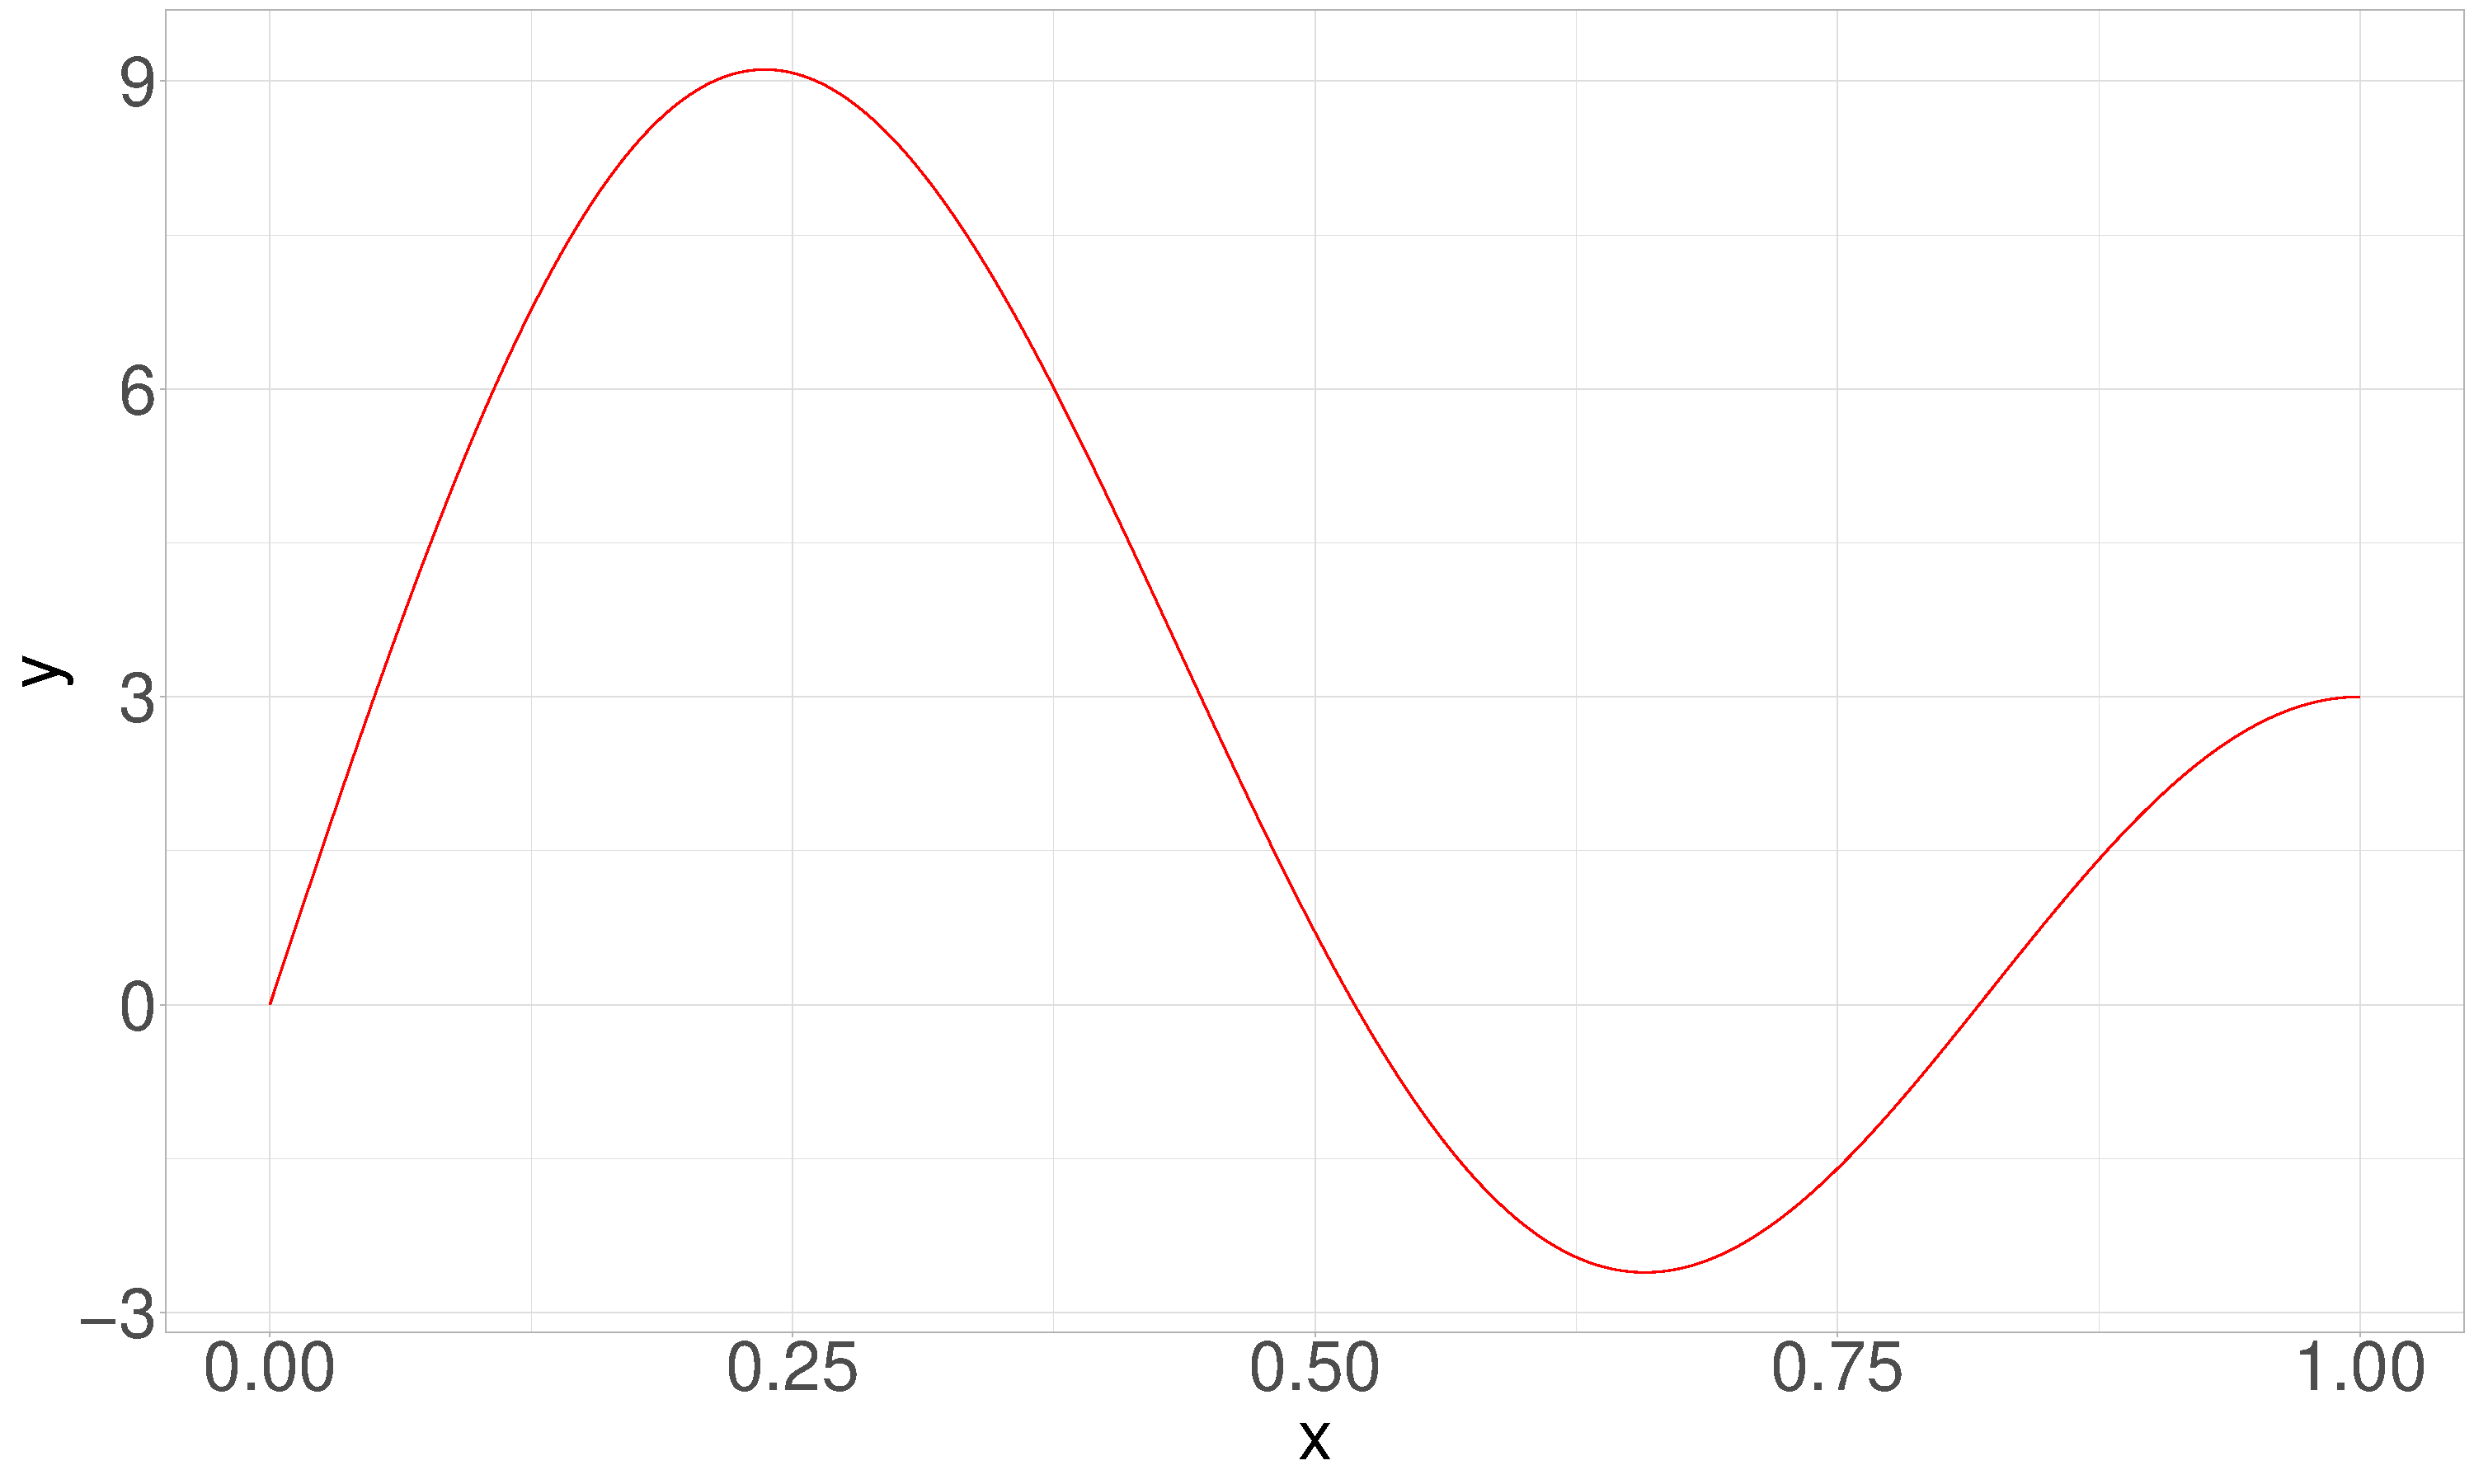
\includegraphics[width=\textwidth]{../Graphics/f1_plot.pdf}
  				\caption{$f_1(t)$, smooth function}
  				\label{fig:test1}
			\end{minipage}%
			\begin{minipage}{.5\textwidth}
	  			\centering
  				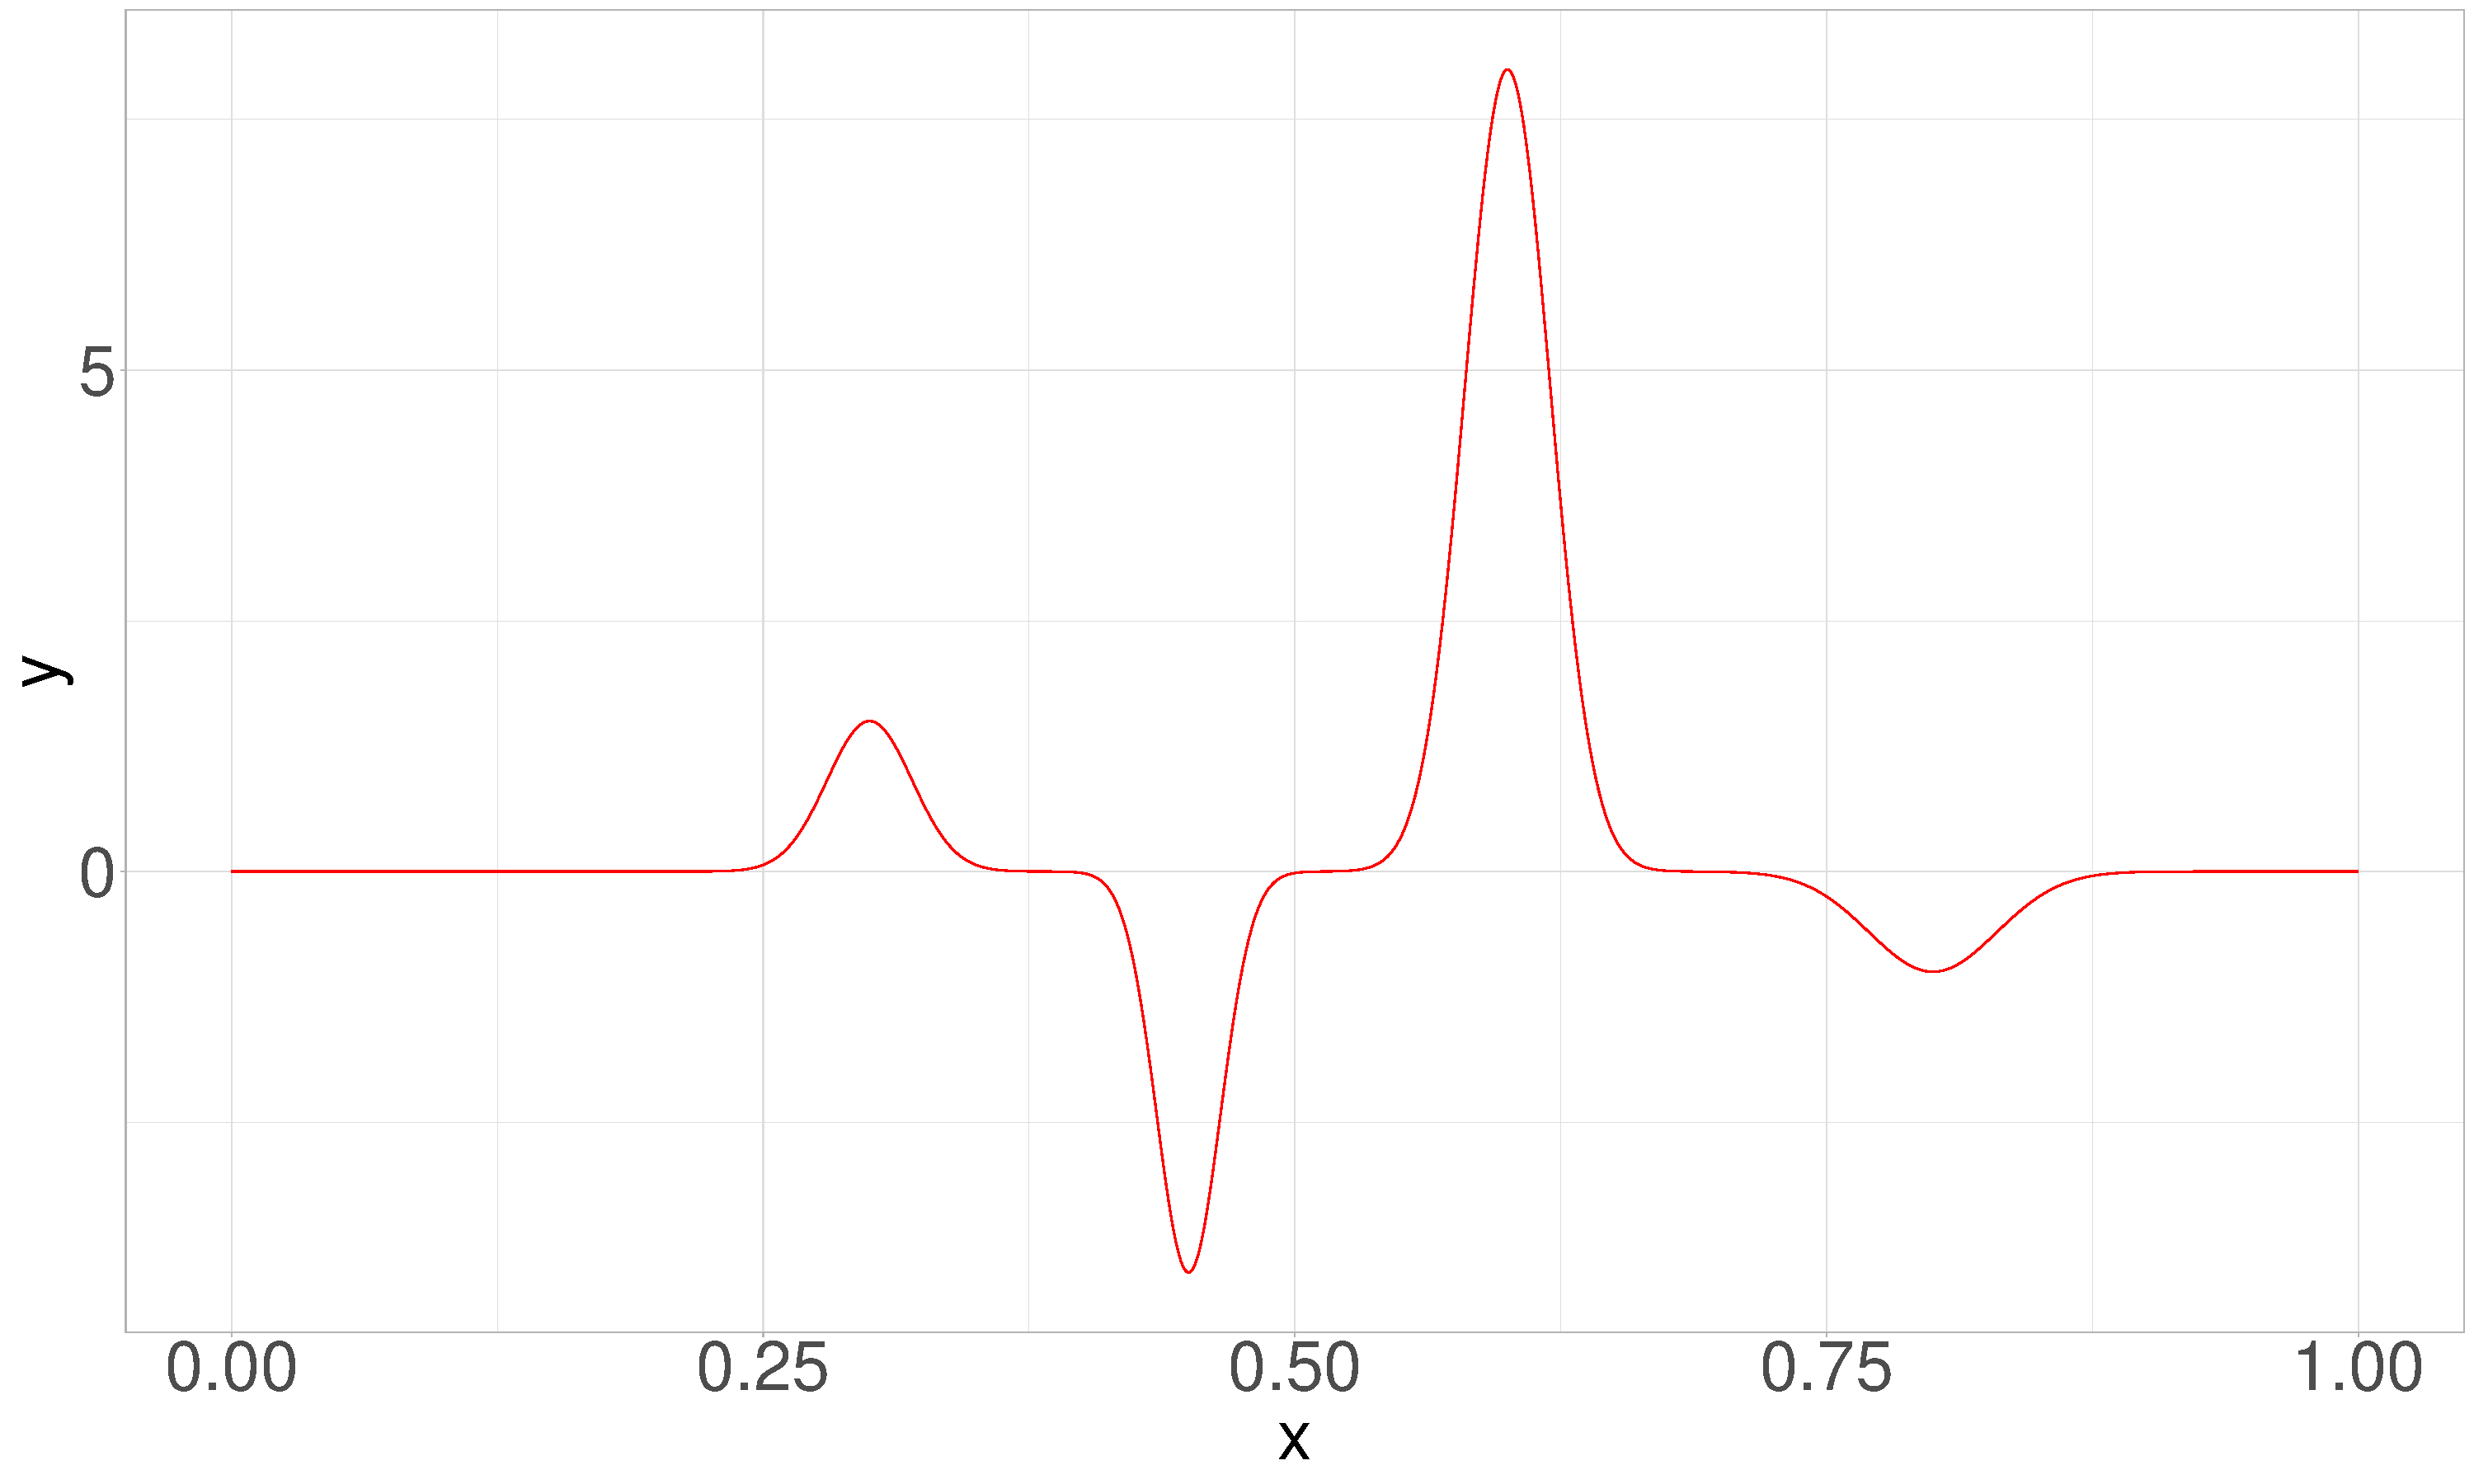
\includegraphics[width=\textwidth]{../Graphics/f2_plot.pdf}
  				\caption{$f_2(t)$, bumpy function}
  				\label{fig:test2}
			\end{minipage}
		\end{figure}
		
		 Two different error-terms $\epsilon$ were created by first generating an $i.i.d.$ standard normal error term and then multiplying it by two error variations $\sigma_e $. The error variations represent different signal-to-noise ratios to test the methods with low and high amounts of noise. They are created such that the squared multiple correlation coefficient $R^2 = var(Xf) / (var(Xf) + \sigma^2_{e})$ is equal to 0.9 and 0.6. The two error terms are then used to generate two sets of responses for $f \in \{f_1(t), f_2(t)\}$
		
		\begin{equation}
			\begin{split}
				Y_{1,f} & = \langle NIR, f\rangle + Z  \biggl\lbrack\frac{var(\langle NIR, f\rangle)}{0.9} - var(\langle NIR, f\rangle)\biggr\rbrack \\
				Y_{2,f} & = \langle NIR, f\rangle + Z  \biggl\lbrack\frac{var(\langle NIR, f\rangle)}{0.6} - var(\langle NIR, f\rangle)\biggr\rbrack
			\end{split}
		\end{equation}
		
		where $Z \sim \mathcal{N}(0,1)$. In total, we created four combinations for the simulations, using the two true coefficient functions and the two sets of responses. These four combinations are then used with a different number of monomial basis functions $ \in \{1,2, \dots, 6\}$, cubic B-spline basis-function $\{5,6,...,18\}$ and Fourier functions $\{1,3,...,25\}$ to predict the generated responses using the basis expansion approach and the FPCR approach. For the evaluation, we used the prediction MSE calculated by 10 fold cross-validation.
		To obtain valid out of sample properties for the FPCR, within each of the ten ten-fold cross-validation splits, we first calculate the first $nharm$ FPC's for $nharm \in \{2,3,4\}$ of the training set $\mathcal{T}$ for each curve $i \in \{1,2, \dots, 200\}$, which was smoothed with the respective basis function specification. The obtained eigenfunctions $\nu^{m,\mathcal{T}}$ are then used to estimate the scores of the holdout set $\mathcal{H}$, $\hat{\xi}_{i}^{m, \mathcal{H}}$  by the equation
		 
		\begin{equation}
			\begin{split}
				\hat{\xi}_{i}^{m, \mathcal{H}} &=  \int_{0}^{1} {\color{red} \left(X_{i}^{\mathcal{H}}(s) - \hat{\mu}^{\mathcal{T}}(s)\right)} {\color{blue}\hat{\nu}^{m, \mathcal{T}} }\mathrm{d}s) 
			    = \int_{0}^{1} {\color{red}\left(\sum_{j \in \mathcal{I}} a_{i,j}^{\mathcal{H}} \phi_j(s)\right)} {\color{blue}\left(\sum_{k \in \mathcal{L}} b_{k}^{m, \mathcal{T}} \psi_{k}(s)\right)} \mathrm{d}s \\
				 &= \sum_{j \in \mathcal{I}} \left[ a_{i,j}^{\mathcal{H}}\sum_{k \in \mathcal{L}}  b_{k}^{m, \mathcal{T}} \int_{0}^{1} \phi_j(s) \psi_{k}(s)\mathrm{d}s\right]
			\end{split}
		\end{equation}
		with truncation parameter $m$.
		\vspace{0.2cm}
	
		 The simulation was done with R (version...). In total, 5000 repetitions were done for each set of simulations. 
		
	\subsection{Results}	
	
	\subsubsection{Basis Expansion Regression}
	The following results origin from the \hyperref[basis_exp_transf]{\textbf{Estimation using Basis-Representation}}, in which we transform the observed functions to perform regression of a scalar on a countable sequence of regressors, which is then tractable with typical multivariate regression theory. 
	
	\paragraph{Monomial Basis}
	Due to the in the number of basis functions increasing collinearity of these basis functions, simulations were conducted up until the sixth monomial basis. For reasons outlined in {\color{green} Link chapter}, they seem suited for $f_1$ and show a better performance than B-splines for this coefficient function, but show the weakest performance for the coefficient function $f_2$. For $f_1$, the simulation selects 5(3) and for $f_2$ 5(5) monomial basis functions for the high(low) signal-to-noise ratios. This weakness is especially pronounced in the setup $f_2,Y_1$; for the high noise setup, $f_2, Y_2$ this weakness is still visible, but less pronounced.
	
	\paragraph{B-spline Basis}
	Simulations with B-spline basis functions were possible from 5 to 18, since from 18 onwards the simulations were running into problems concerning {\color{green} what happened here exactly?}
	The smooth function $f_1$ requires only 5(4) B-spline basis functions, for the high(low) signal-to-noise ratio to obtain the best fit for the B-spline basis, which performs the worst for $f_1$. For $f_2$, 11(6) B-spline basis functions are needed for the high(low) signal-to-noise ratios. For $f_2$, the B-spline basis functions outperform the monomial basis but come second to the Fourier basis.
	
	\paragraph{Fourier Basis}
	For $f_1$, the simulation chooses a smaller number of Fourier basis functions, 5(3) and a higher number for the bumpy function $f_2$, 9(7) for the setup with the high(low) signal-to-noise ratio. With the low signal-to-noise ratio, the simulation chooses a smaller number to account for the higher noise in the response variable. The Fourier basis functions perform the best in each setup for the basis expansion regression. When recalling $f_1$ and $f_2$, both, but especially $f_1$ shows similar curvature order across the domain which contributes to the strong performance of this basis.	\\
	
	For all specifications, the effect of the Bias-Variance tradeoff can be observed: The function $f_1$ is rather smooth and little bias introduced when choosing a small number of basis functions. For $f_2$, higher number of basis functions are needed, resulting from the inherent peculiarities of $f_2$. We can choose a higher number of basis functions since the amount of bias is decreasing faster in the number of basis functions than the variance is increasing compared to $f_1$. 

	\subsubsection{Functional Principal Component Regression}
	The model which is used for the FPCR is described in \hyperref[fpc_exp_transf]{\textbf{Estimation using Functional Principal Components}}. Additionally to the selection of the truncation parameter $K$, the choice of the number of FPC's adds to the complexity of the model since the eigenvalues and -functions from the decomposition are influenced by the choice of $K$ that was used to approximate the function.
	
	\paragraph{Monomial Basis}
	TBD
	\paragraph{B-spline Basis}
	For $f_1,Y_1$, the CV suggests a better model with a higher number of FPC's. While the number of basis functions stays at five for two and three used FPC, it increases to six basis functions for $nharm$ = 4. In $f_1,Y_1$, the cross-validated MSE is only slightly affected by the number of FPC's, but lowest for $nharm$ = 3, indicating the possibility of over-fitting for four FPC's. $f_2,Y_1$ shows the strongest decrease of MSE in increasing FPC's of all FPCR models fitted with B-splines (0.69614, 0.42504, 0.09497 for 2,3,4 FPC's). For $f_2,Y_2$ the same holds true as in the setup with $f_2$ and the high signal-to-noise ratio, but less pronounced. Similar to the two setups with $f_1$, the cross-validated number of basis functions is increasing in the number of FPC's (4,6,8 for 2,3,4 FPC's)\\
	The results overall might indicate that a higher number of FPC's has a strong effect in the setup with a high signal-to-noise ratio while not reducing as much error in the setting with the higher noise.
	
	\paragraph{Fourier Basis}
	We observe similar behavior as for the FPCR using B-splines. In $f_1,Y_1$, the MSE is decreasing in the number of FPC's while the results in $f_1,Y_2$ might indicate overfitting when using four FPC's. Since it was not possible to calculate the cross-validated MSE for three basis functions for four FPC's, the increasing number of basis functions as seen in the FPCR with B-splines can not be observed here. $f_2,Y_1$ displays the greatest decline of MSE in the increasing number of FPC's. The same behavior can be seen in $f_2,Y_2$, but less pronounced. Both configurations of $f_2$ are using 5,15,7 basis functions for 2,3,4 FPC's: This behavior opposes to the previously reported increasing nature of basis functions in the number of FPC's.
	
	\subsubsection{Interpretation and Relevance for Application}
	
	%\subsection{Literature}
	%\begin{itemize}
	%	\item \cite{shonkwiler_explorations_2009}
	%	\item R-packages: fda, refund, mgcv
	%\end{itemize}

	\section{Application}\label{Application}
		The application uses the methods from the previous sections to predict the octane ratings of the introduced gasoline dataset. The simulation study will contribute towards the reading of the results. 
		\begin{itemize}
			\item {\color{green} incorporate results of simulation study: 					number of basis, components, etc...}
			\item point out difficulties estimating sderror
			\item describe setup and results
		\end{itemize}
	
	\subsection{Literature}
	\begin{itemize}
		\item \cite{carey_life_2002}
	\end{itemize}

	\section{Outlook}\label{Outlook}
	
	\subsection{Literature}
	\begin{itemize}
		\item \cite{James.2009} (shape-restrictions)
	\end{itemize}
	
	\newpage
	\section{Appendix}
	
	\subsection{Near-infrared (NIR) Spectroscopy}
	NIR- spectroscopy is a spectroscopic method that uses the near-infrared region of the electromagnetic spectrum (From 780 nm to 2500 nm). It, therefore, measures the absorption and interaction of this spectrum of radiation with the sample. NIR-spectroscopy is not only faster and cheaper than the standard test procedure – another significant advantage is that it does not need a reagent and thus does not destroy the sample. It is used for analysis in different sectors and fields, like the agrochemical industry and healthcare. Its non-invasive nature makes it also an asset for medical applications like the monitoring of diabetes in which NIR-spectroscopy can detect the worsening of the blood glucose metabolic dysfunction (cf . \cite{FR_li_et_al_2020}). \\
	In the context of this paper, the gasoline dataset which is used for the simulation and the application is constructed using NIR spectroscopy. According to \cite{Bohacs_Ovadi_Salgo1998} NIR-spectroscopy is a feasible method for the analysis of gasoline since most of the absorption that is observed within the described interval of wavelengths is due to overtones and interactions of the radiation with chemical combinations (carbon–hydrogen, carbon–carbon, carbon–oxygen, carbonyl associated groups, aromatic stretching, and deformation vibration of the hydrocarbon molecules). While this paper focuses on the prediction of the octane number of gasoline, other research focuses  on different properties of gasoline such as the olefin, naphtaenic and aromatic content (Parisi et al. 1990, as cited in \cite{Bohacs_Ovadi_Salgo1998}) or the distillation characteristics (Pauls 1985, as cited in \cite{Bohacs_Ovadi_Salgo1998})

	\begin{figure}[H]
		\begin{center}
			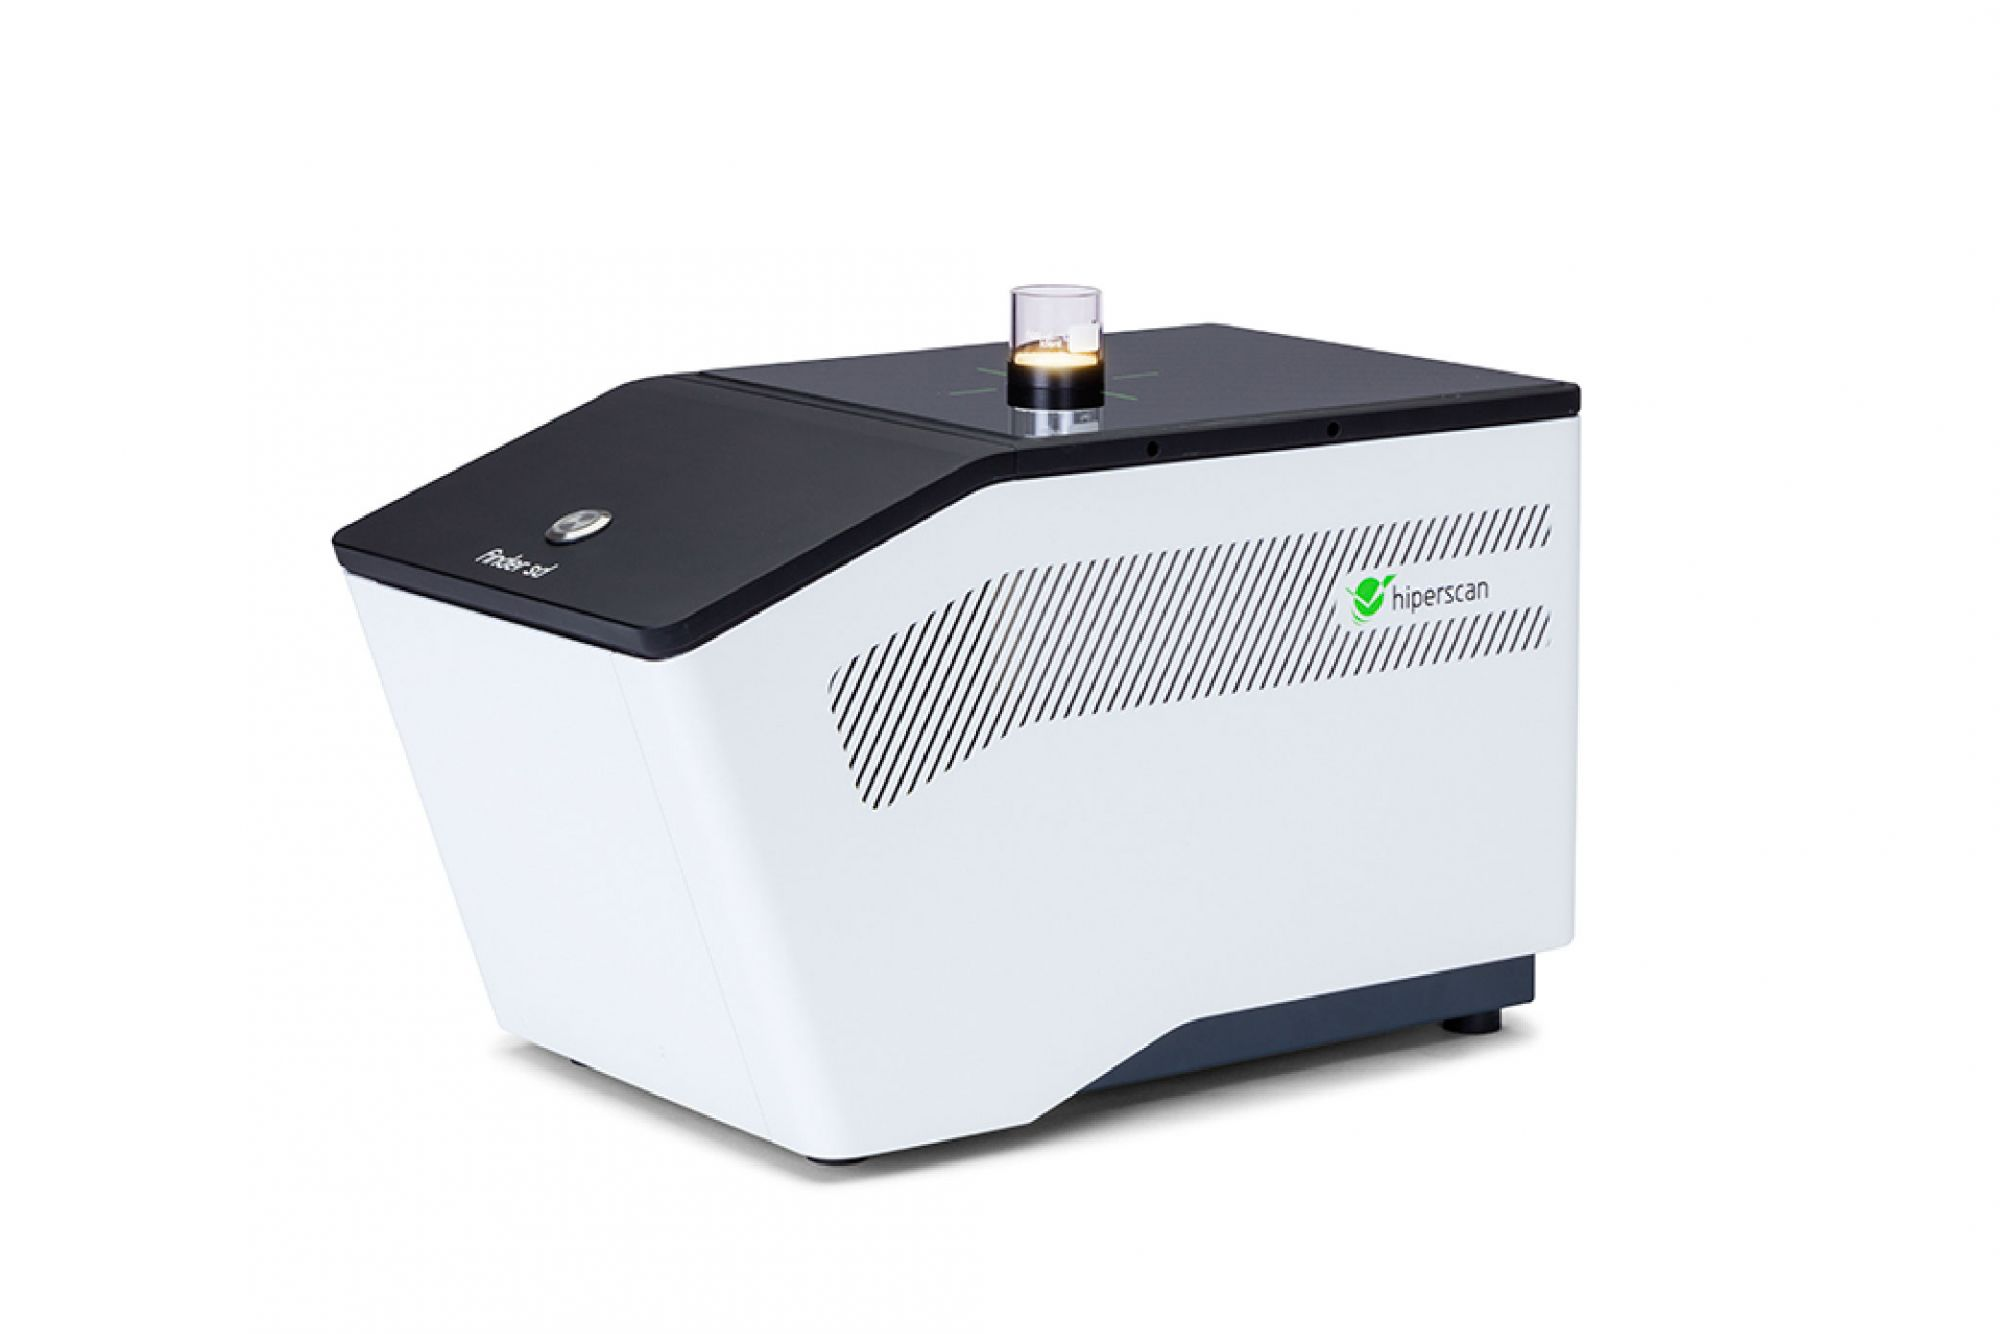
\includegraphics[width = \textwidth]{../Graphics/FinderSD.jpg}
			\caption{Finder SD - A Near-Infrared-Spectroscope built by HiperScan GmbH \\
			(Source: https://www.hiperscan.com/files/apoident/uploads/Bilder/Neue\_Website/Produkte/FinderSD.jpg)}
		\end{center}
	\end{figure}

	\newpage
	
	\subsection{Basis Plots}
	
	\begin{figure}[H]\label{Fourier_basis}
		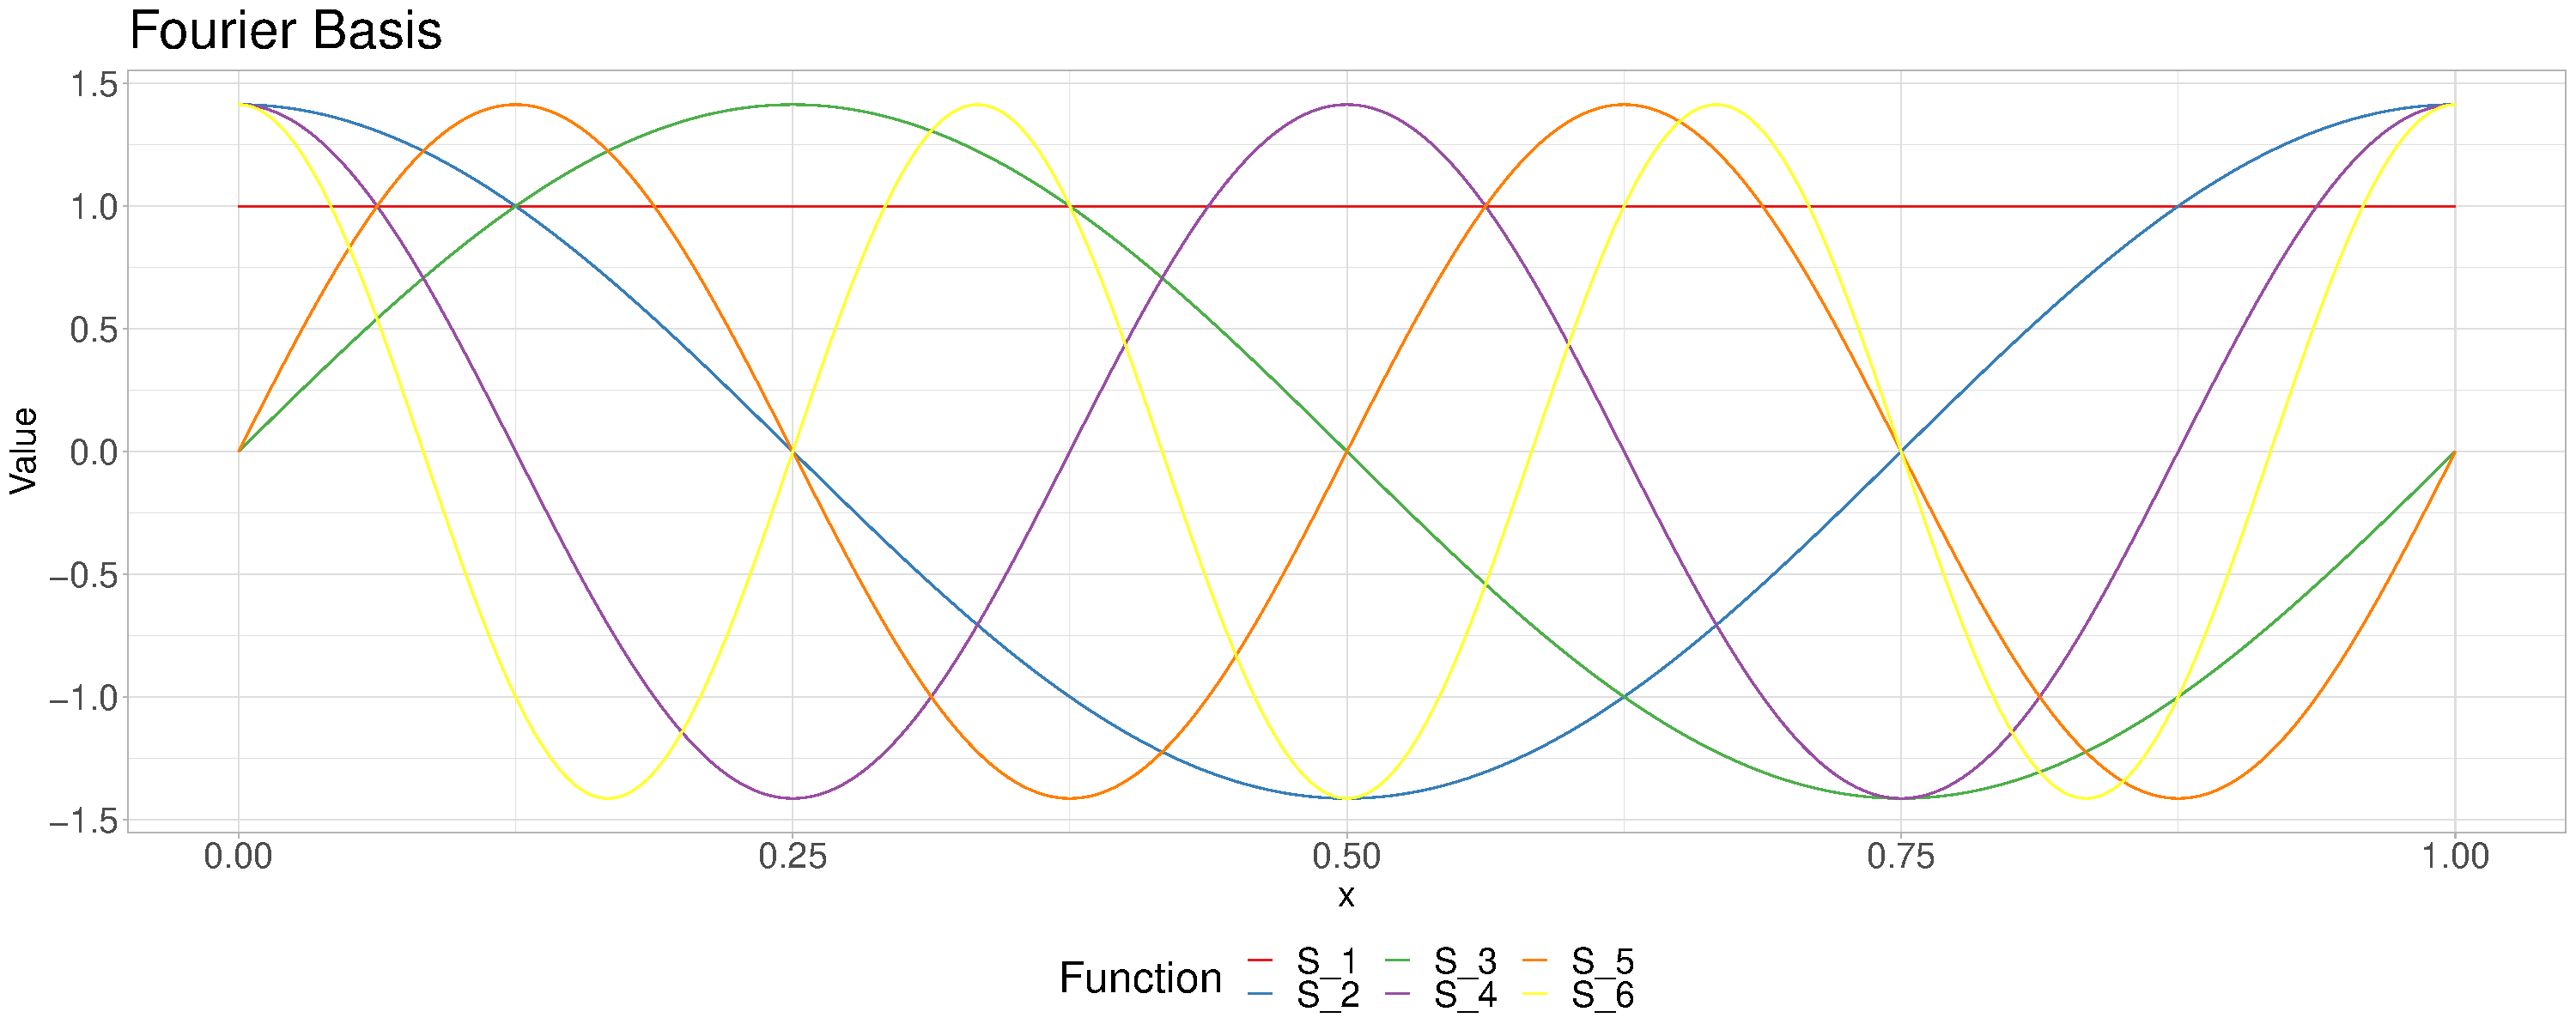
\includegraphics[width = \textwidth]{../Graphics/Fourier_Basis.pdf}
		\caption{Fourier basis functions for $i = 1,\dots,7$}
	\end{figure}
	
	\begin{figure}[H]\label{B-spline_basis}
		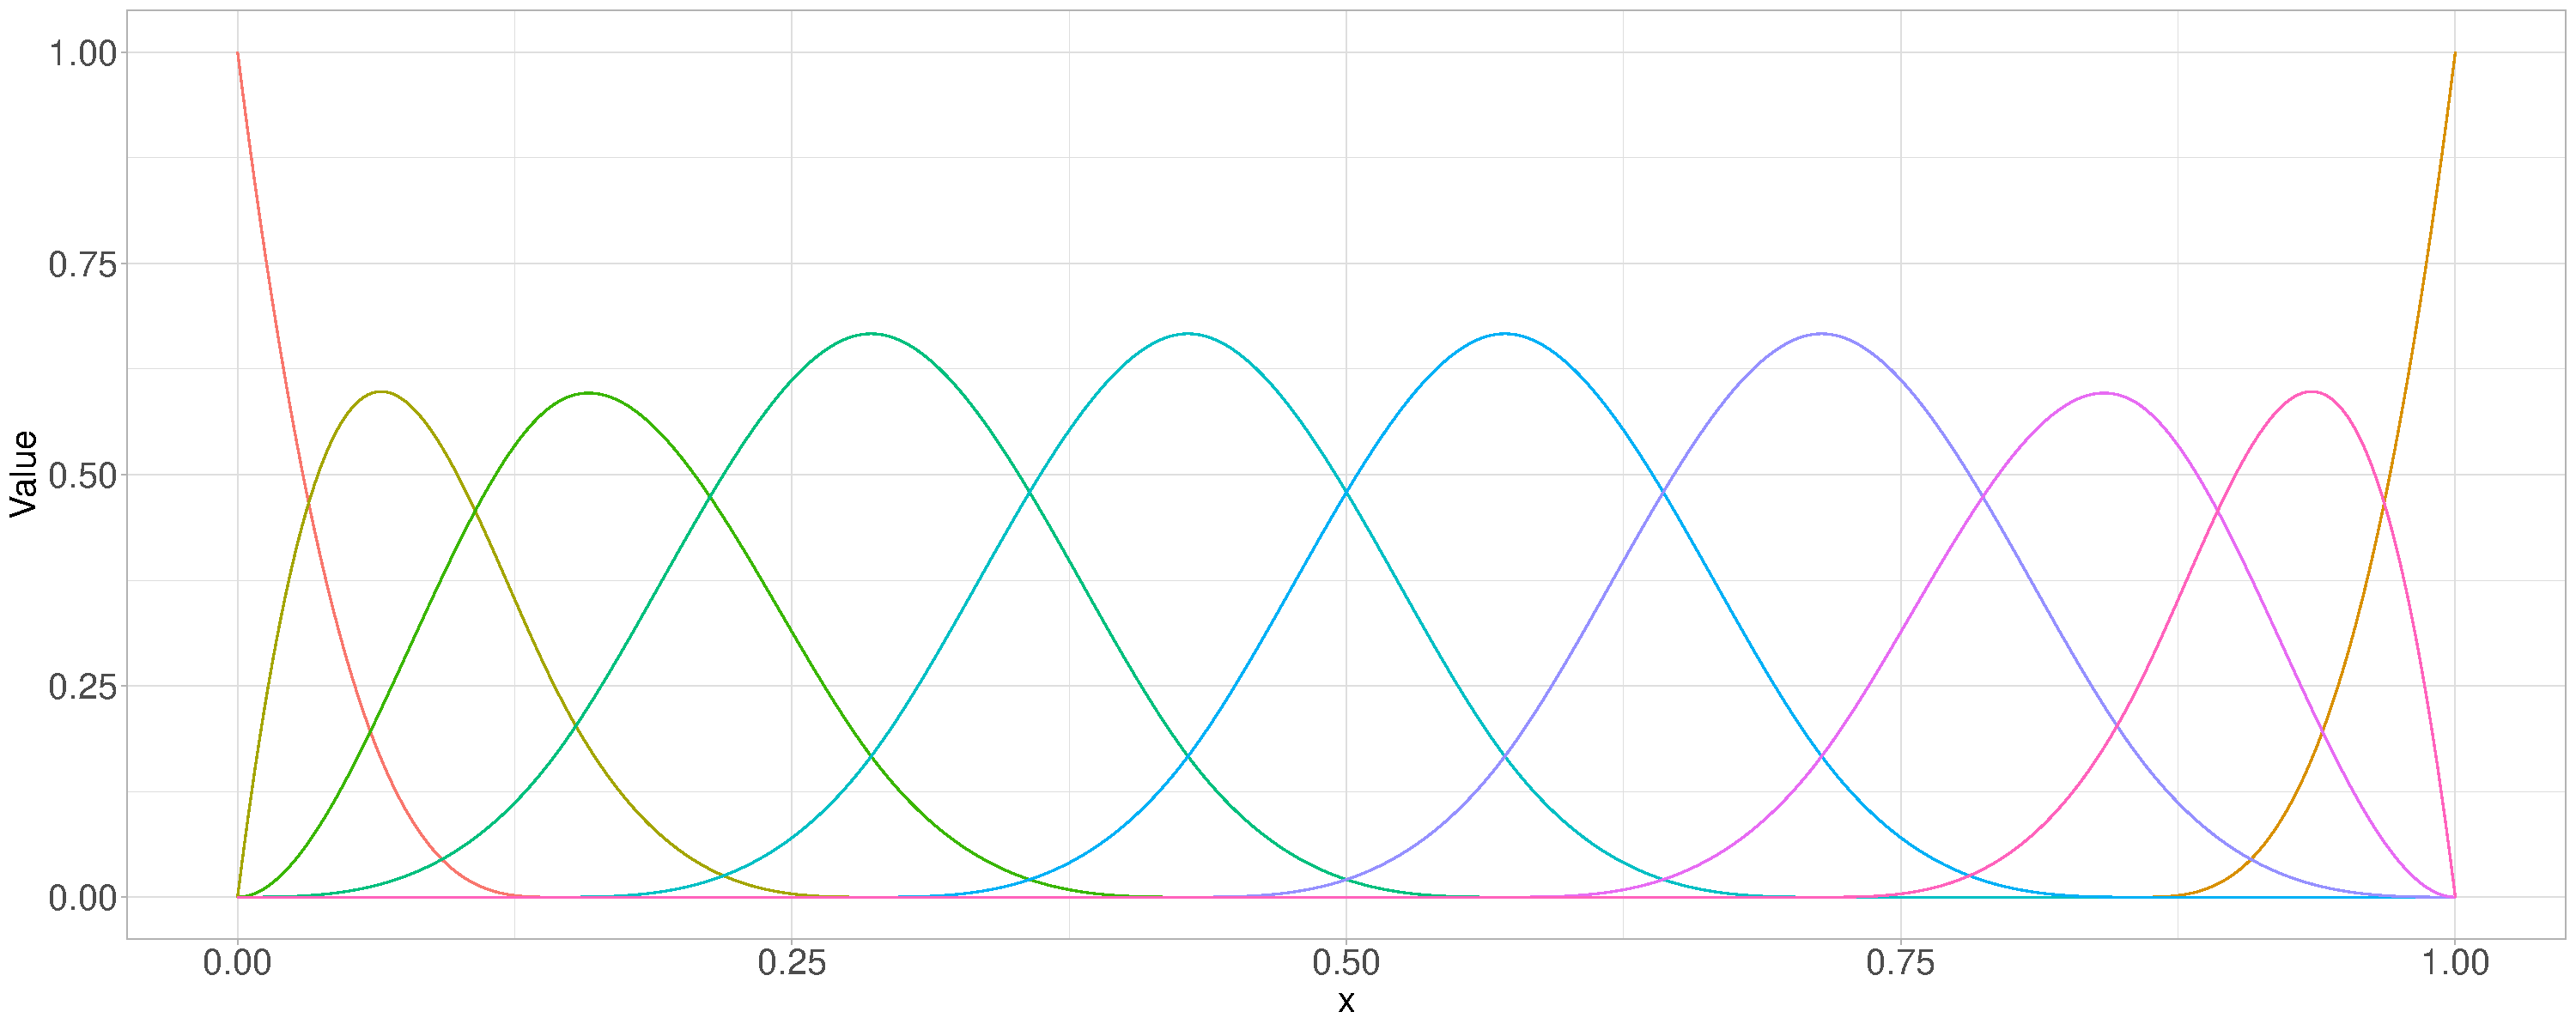
\includegraphics[width = \textwidth]{../Graphics/Bspline_Basis.pdf}
		\caption{B-spline basis functions of order 4 for 8 equidistant knots on $[0,1]$}
	\end{figure}

	\begin{figure}[H]\label{monomial_basis}
		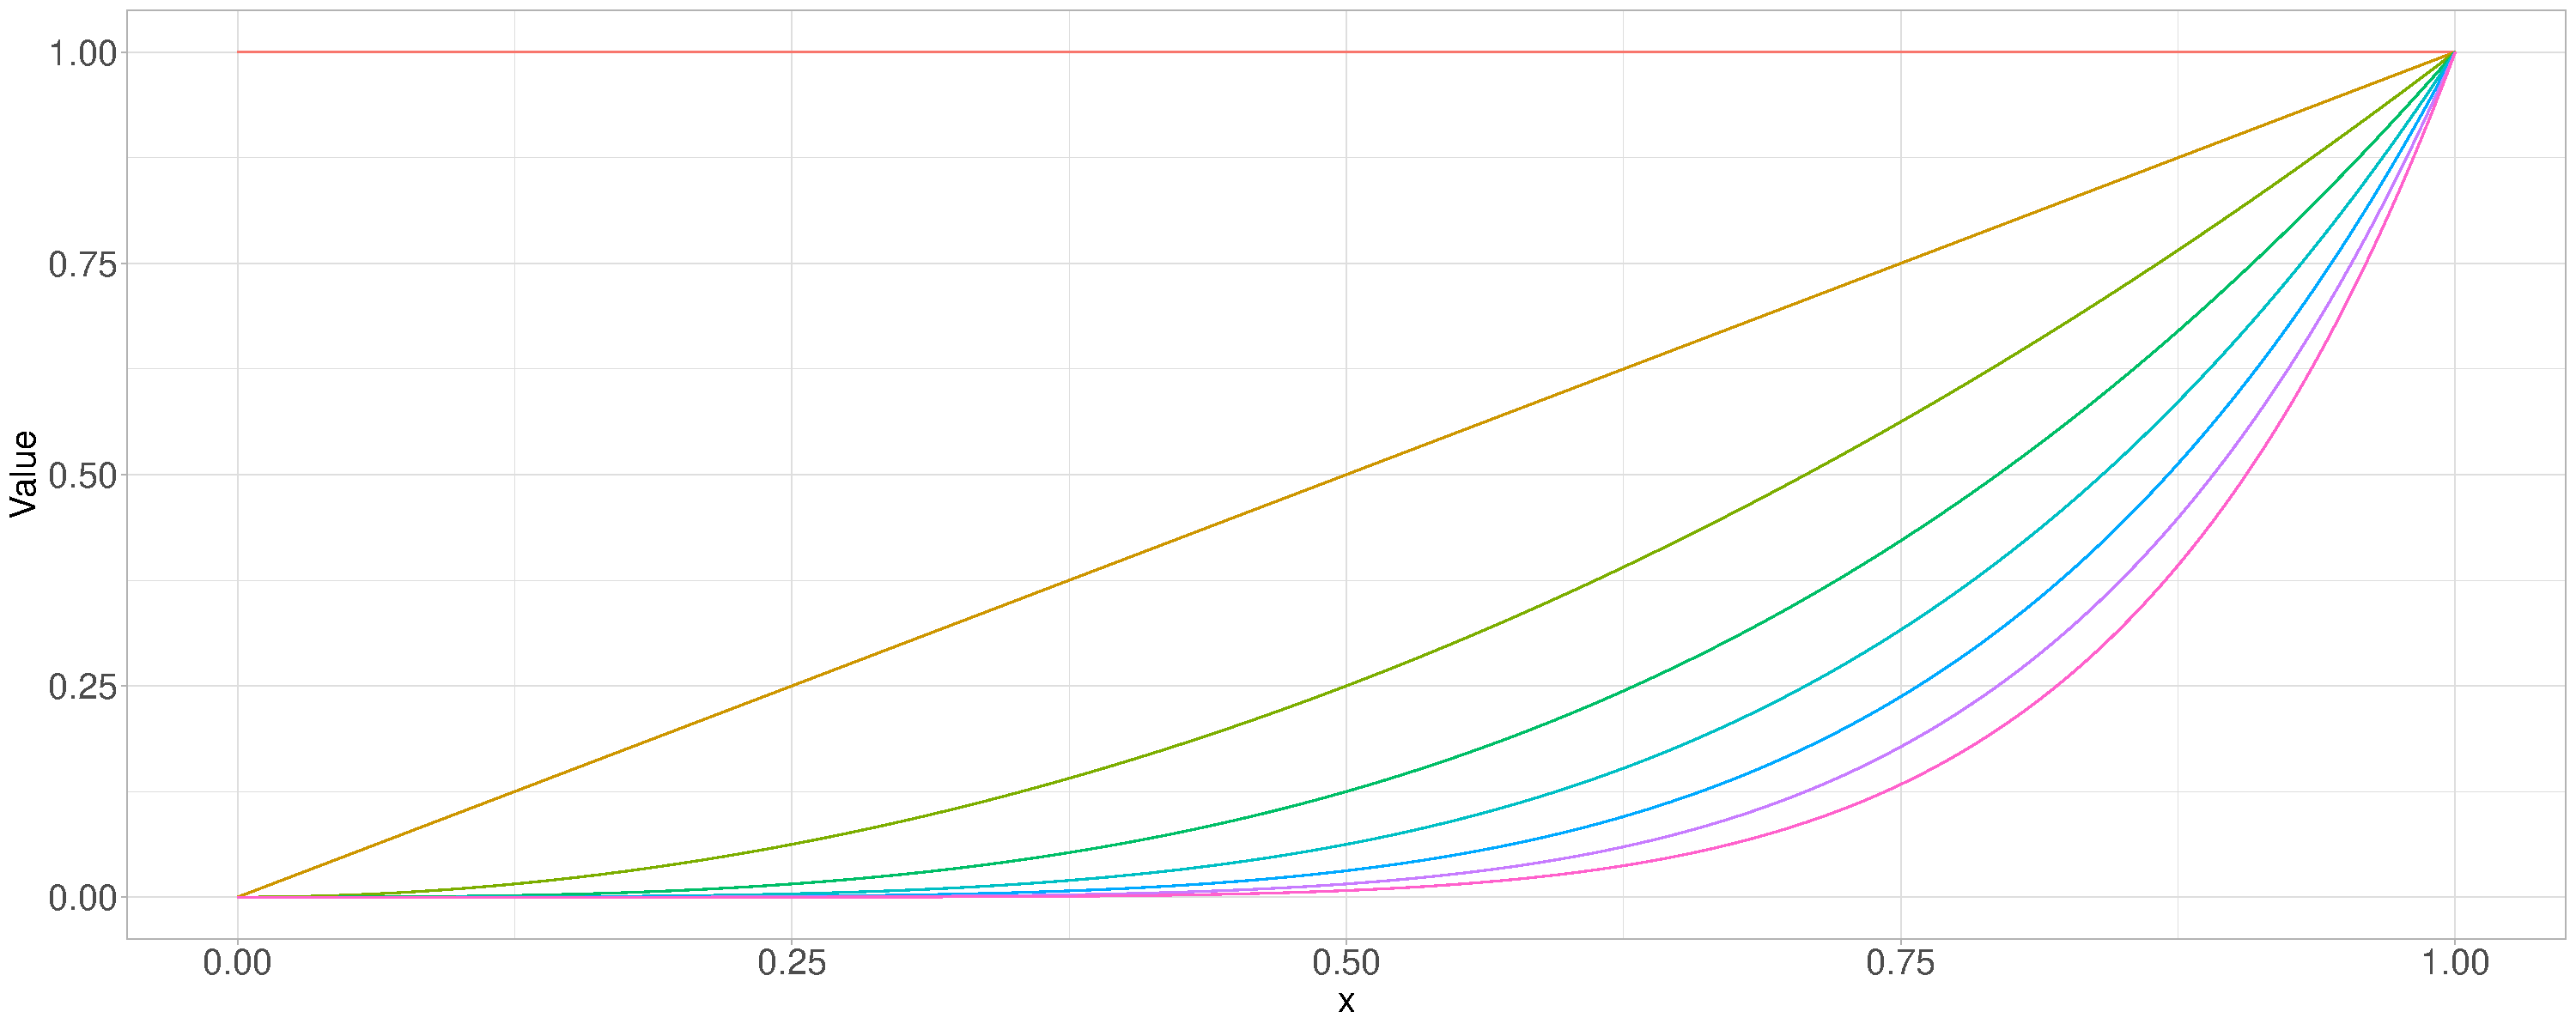
\includegraphics[width = \textwidth]{../Graphics/Monomial_Basis.pdf}
		\caption{Monomial basis functions of degree 0 to 7}
	\end{figure}

\newpage
% extrernal file for all tables Tables


\subsection{Simulation Study Results}
	

	\begin{table}[htb]
			\centering
			\caption{Monomial Basis Expansion Regression}
				\begin{tabular}{lllllll}
					\cline{1-5}
					 \boldmath{$f_1, Y_1$}                 & \boldmath{$f_1, Y_2$}                  & \boldmath{$f_2, Y_1$}                    & \boldmath{$f_2, Y_2$}               & \textbf{n\_basis} &  \\ \cline{1-5}
7.17723                       & 131.92717                        & 0.89367                        & 2.58395                        & 2       \\
4.17039                       & {\color[HTML]{FE0000} 129.64259} & 0.81224                        & 2.51177                        & 3       \\
3.91275                       & 130.11708                        & 0.38079                        & 2.09047                        & 4       \\
{\color[HTML]{FE0000} 3.6385} & 130.59817                        & {\color[HTML]{FE0000} 0.09217} & {\color[HTML]{FE0000} 1.81343} & 5       \\
6.01644                       & 201.15535                        & 0.76208                        & 3.39373                        & 6      
\end{tabular}
\end{table}

\vspace{0.5cm}


	\begin{table}[htb]
			\centering
			\caption{BSpline Basis Expansion Regression}
				\begin{tabular}{lllllll}
					\cline{1-5}
					 \boldmath{$f_1, Y_1$}                 & \boldmath{$f_1, Y_2$}                  & \boldmath{$f_2, Y_1$}                    & \boldmath{$f_2, Y_2$}               & \textbf{n\_basis} &  \\ \cline{1-5}
3.91275                        & {\color[HTML]{FE0000} 130.11708} & 0.38079                       & 2.09047                        & 4       \\
{\color[HTML]{FE0000} 3.64305} & 130.61095                        & 0.09512                       & 1.81643                        & 5       \\
3.65426                        & 131.35355                        & 0.07775                       & {\color[HTML]{FE0000} 1.80913} & 6       \\
3.67705                        & 132.14205                        & 0.07518                       & 1.8168                         & 7       \\
3.71074                        & 133.36537                        & 0.0581                        & 1.8165                         & 8       \\
3.71921                        & 133.68149                        & 0.0564                        & 1.81931                        & 9       \\
3.74201                        & 134.51217                        & 0.05218                       & 1.82576                        & 10      \\
3.7644                         & 135.29727                        & {\color[HTML]{FE0000} 0.0519} & 1.8361                         & 11      \\
3.80109                        & 136.57581                        & 0.05204                       & 1.85315                        & 12      \\
3.83436                        & 137.78407                        & 0.05271                       & 1.86997                        & 13      \\
3.86217                        & 138.73431                        & 0.05307                       & 1.88269                        & 14      \\
3.86856                        & 138.97427                        & 0.0526                        & 1.88482                        & 15      \\
3.88506                        & 139.57419                        & 0.05283                       & 1.89335                        & 16      \\
3.91267                        & 140.5149                         & 0.05322                       & 1.90619                        & 17      \\
3.94813                        & 141.80885                        & 0.05358                       & 1.92312                        & 18     
\end{tabular}
\end{table}


\vspace{0.5cm}


	\begin{table}[htb]
			\centering
			\caption{Fourier Basis Expansion Regression}
				\begin{tabular}{lllllll}
					\cline{1-5}
					 \boldmath{$f_1, Y_1$}                 & \boldmath{$f_1, Y_2$}                  & \boldmath{$f_2, Y_1$}                    & \boldmath{$f_2, Y_2$}               & \textbf{n\_basis} &  \\ \cline{1-5}
3.69752                       & {\color[HTML]{FE0000} 129.19134} & 0.69524                        & 2.3944                         & 3       \\
{\color[HTML]{FE0000} 3.6347} & 130.59282                        & 0.07418                        & 1.79582                        & 5       \\
3.67623                       & 132.08248                        & 0.05147                        & {\color[HTML]{FE0000} 1.79343} & 7       \\
3.71885                       & 133.67575                        & {\color[HTML]{FE0000} 0.05105} & 1.81291                        & 9       \\
3.76451                       & 135.26219                        & 0.05146                        & 1.83463                        & 11      \\
3.81095                       & 136.90282                        & 0.05197                        & 1.85724                        & 13      \\
3.85674                       & 138.57258                        & 0.05252                        & 1.88021                        & 15      \\
3.90619                       & 140.29178                        & 0.05304                        & 1.90283                        & 17      \\
3.95517                       & 142.05727                        & 0.05365                        & 1.92718                        & 19     
\end{tabular}
\end{table}

\vspace{0.5cm}

%%%%%%%%%%%%%%%%%%%%%%%%%%%%%%%%
% Monomial FPCR
%%%%%%%%%%%%%%%%%%%%%%%%%%%%%%%%




%%%%%%%%%%%%%%%%%%%%%%%%%%%%%%%%
% Bspline FPCR
%%%%%%%%%%%%%%%%%%%%%%%%%%%%%%%%

	\begin{table}[htb]
			\centering
			\caption{BSpline FPCR, $nharm$ = 2}
				\begin{tabular}{lllllll}
					\cline{1-5}
					 \boldmath{$f_1, Y_1$}                 & \boldmath{$f_1, Y_2$}                  & \boldmath{$f_2, Y_1$}                    & \boldmath{$f_2, Y_2$}               & \textbf{n\_basis} &  \\ \cline{1-5}
10.93556                       & 135.66335                        & {\color[HTML]{FE0000} 0.69614} & {\color[HTML]{FE0000} 2.38597} & 4       \\
{\color[HTML]{FE0000} 6.01366} & {\color[HTML]{FE0000} 130.75986} & 0.77796                        & 2.46801                        & 5       \\
6.36762                        & 131.10562                        & 0.79035                        & 2.48029                        & 6       \\
6.76471                        & 131.49507                        & 0.7684                         & 2.45834                        & 7       \\
7.21393                        & 131.93622                        & 0.7958                         & 2.48568                        & 8       \\
7.77885                        & 132.48984                        & 0.75447                        & 2.44437                        & 9       \\
8.48517                        & 133.18046                        & 0.71664                        & 2.40654                        & 10      \\
8.95142                        & 133.63714                        & 0.70481                        & 2.39475                        & 11      \\
9.21314                        & 133.89421                        & 0.71456                        & 2.4045                         & 12      \\
9.29854                        & 133.97794                        & 0.73961                        & 2.42952                        & 13      \\
9.31792                        & 133.99732                        & 0.74046                        & 2.43037                        & 14      \\
9.32858                        & 134.00809                        & 0.74354                        & 2.43344                        & 15      \\
9.27722                        & 133.95811                        & 0.77399                        & 2.46383                        & 16      \\
9.23813                        & 133.91976                        & 0.77175                        & 2.46159                        & 17      \\
9.33983                        & 134.01705                        & 0.76653                        & 2.45632                        & 18      \\
9.24067                        & 133.92097                        & 0.78389                        & 2.47367                        & 19      \\
9.34246                        & 134.01837                        & 0.75304                        & 2.44285                        & 20      \\
9.38735                        & 134.06288                        & 0.76148                        & 2.45127                        & 21      \\
9.35218                        & 134.02839                        & 0.75842                        & 2.44823                        & 22      \\
9.50715                        & 134.17875                        & 0.74067                        & 2.43049                        & 23      \\
9.51344                        & 134.18666                        & 0.7552                         & 2.44502                        & 24      \\
9.52277                        & 134.19463                        & 0.75125                        & 2.44107                        & 25     
\end{tabular}
\end{table}

\vspace{0.5cm}


	\begin{table}[htb]
			\centering
			\caption{BSpline FPCR, $nharm$ = 3}
				\begin{tabular}{lllllll}
					\cline{1-5}
					 \boldmath{$f_1, Y_1$}                 & \boldmath{$f_1, Y_2$}                  & \boldmath{$f_2, Y_1$}                    & \boldmath{$f_2, Y_2$}               & \textbf{n\_basis} &  \\ \cline{1-5}
4.26915                        & 129.73814                        & 0.65618                        & 2.35517                      & 4       \\
{\color[HTML]{FE0000} 3.99153} & {\color[HTML]{FE0000} 129.47951} & 0.75902                        & 2.45877                      & 5       \\
4.13265                        & 129.64227                        & {\color[HTML]{FE0000} 0.42504} & {\color[HTML]{FE0000} 2.126} & 6       \\
4.15027                        & 129.66158                        & 0.52603                        & 2.22684                      & 7       \\
4.28266                        & 129.7862                         & 0.71107                        & 2.41134                      & 8       \\
4.30464                        & 129.8084                         & 0.65968                        & 2.36019                      & 9       \\
4.32579                        & 129.82882                        & 0.60062                        & 2.3013                       & 10      \\
4.29797                        & 129.80089                        & 0.65658                        & 2.35703                      & 11      \\
4.32782                        & 129.82922                        & 0.68072                        & 2.38108                      & 12      \\
4.34042                        & 129.84041                        & 0.71583                        & 2.41605                      & 13      \\
4.3526                         & 129.8512                         & 0.72262                        & 2.42279                      & 14      \\
4.3577                         & 129.85642                        & 0.72621                        & 2.42637                      & 15      \\
4.37694                        & 129.87493                        & 0.75746                        & 2.45749                      & 16      \\
4.35973                        & 129.85893                        & 0.75291                        & 2.45296                      & 17      \\
4.37223                        & 129.87141                        & 0.69875                        & 2.39878                      & 18      \\
4.34433                        & 129.84395                        & 0.74346                        & 2.44353                      & 19      \\
4.36545                        & 129.86595                        & 0.67405                        & 2.37412                      & 20      \\
4.36942                        & 129.86886                        & 0.67941                        & 2.37944                      & 21      \\
4.34272                        & 129.843                          & 0.6919                         & 2.39205                      & 22      \\
4.38437                        & 129.88403                        & 0.64702                        & 2.34708                      & 23      \\
4.35012                        & 129.8495                         & 0.68435                        & 2.38446                      & 24      \\
4.36866                        & 129.86795                        & 0.67512                        & 2.37514                      & 25     
\end{tabular}
\end{table}


\vspace{0.5cm}}


	\begin{table}[htb]
			\centering
			\caption{BSpline FPCR, $nharm$ = 4}
				\begin{tabular}{lllllll}
					\cline{1-5}
					 \boldmath{$f_1, Y_1$}                 & \boldmath{$f_1, Y_2$}                  & \boldmath{$f_2, Y_1$}                    & \boldmath{$f_2, Y_2$}               & \textbf{n\_basis} &  \\ \cline{1-5}
3.91274                        & 130.1171                         & 0.38077                        & 2.09045                       & 4       \\
3.97061                        & 130.18108                        & 0.75664                        & 2.46627                       & 5       \\
{\color[HTML]{FE0000} 3.83646} & {\color[HTML]{FE0000} 130.05682} & 0.19244                        & 1.90433                       & 6       \\
3.8814                         & 130.0934                         & 0.3326                         & 2.04419                       & 7       \\
4.2679                         & 130.49905                        & {\color[HTML]{FE0000} 0.09497} & {\color[HTML]{FE0000} 1.8071} & 8       \\
4.31978                        & 130.54252                        & 0.15828                        & 1.87039                       & 9       \\
4.32413                        & 130.5527                         & 0.10538                        & 1.81745                       & 10      \\
4.31263                        & 130.53896                        & 0.13116                        & 1.84322                       & 11      \\
4.33997                        & 130.56608                        & 0.10762                        & 1.81971                       & 12      \\
4.34107                        & 130.56642                        & 0.11868                        & 1.83076                       & 13      \\
4.35627                        & 130.57893                        & 0.12832                        & 1.84037                       & 14      \\
4.35369                        & 130.57747                        & 0.11173                        & 1.82379                       & 15      \\
4.35313                        & 130.57695                        & 0.11652                        & 1.82861                       & 16      \\
4.3476                         & 130.57119                        & 0.11283                        & 1.82497                       & 17      \\
4.31541                        & 130.54208                        & 0.08832                        & 1.80044                       & 18      \\
4.32121                        & 130.54666                        & 0.10087                        & 1.81304                       & 19      \\
4.2968                         & 130.52361                        & 0.08341                        & 1.79552                       & 20      \\
4.30044                        & 130.52787                        & 0.08785                        & 1.79994                       & 21      \\
4.29859                        & 130.52514                        & 0.08833                        & 1.80045                       & 22      \\
4.28391                        & 130.51071                        & 0.08189                        & 1.79394                       & 23      \\
4.29418                        & 130.52054                        & 0.08928                        & 1.80134                       & 24      \\
4.28911                        & 130.51512                        & 0.0856                         & 1.79766                       & 25     
\end{tabular}
\end{table}
\vspace{0.5cm}

%%%%%%%%%%%%%%%%%%%%%%%%%%%%%%%%
% Fourier FPCR
%%%%%%%%%%%%%%%%%%%%%%%%%%%%%%%%

	\begin{table}[htb]
			\centering
			\caption{Fourier FPCR, $nharm$ = 2}
				\begin{tabular}{lllllll}
					\cline{1-5}
					 \boldmath{$f_1, Y_1$}                 & \boldmath{$f_1, Y_2$}                  & \boldmath{$f_2, Y_1$}                    & \boldmath{$f_2, Y_2$}               & \textbf{n\_basis} &  \\ \cline{1-5}
{\color[HTML]{FE0000} 5.04859} & {\color[HTML]{FE0000} 129.81003} & 0.78889                        & 2.4789                         & 3       \\
5.08647                        & 129.84459                        & {\color[HTML]{FE0000} 0.69756} & {\color[HTML]{FE0000} 2.38778} & 5       \\
5.29235                        & 130.04946                        & 0.80393                        & 2.49395                        & 7       \\
5.32414                        & 130.07859                        & 0.80074                        & 2.49072                        & 9       \\
5.34403                        & 130.09777                        & 0.79714                        & 2.48713                        & 11      \\
5.43601                        & 130.18816                        & 0.8141                         & 2.50404                        & 13      \\
5.51333                        & 130.26036                        & 0.78908                        & 2.47902                        & 15      \\
5.70153                        & 130.44275                        & 0.79659                        & 2.48646                        & 17      \\
5.87259                        & 130.6101                         & 0.77783                        & 2.46771                        & 19     
\end{tabular}
\end{table}

\vspace{0.5cm}


	\begin{table}[htb]
			\centering
			\caption{Fourier FPCR, $nharm$ = 3}
				\begin{tabular}{lllllll}
					\cline{1-5}
					 \boldmath{$f_1, Y_1$}                 & \boldmath{$f_1, Y_2$}                  & \boldmath{$f_2, Y_1$}                    & \boldmath{$f_2, Y_2$}               & \textbf{n\_basis} &  \\ \cline{1-5}
{\color[HTML]{FE0000} 3.69752} & {\color[HTML]{FE0000} 129.19134} & 0.69524                        & 2.3944                         & 3       \\
5.06895                        & 130.54881                        & 0.1376                         & 1.83947                        & 5       \\
5.21758                        & 130.69839                        & 0.13994                        & 1.84156                        & 7       \\
5.22636                        & 130.70697                        & 0.12715                        & 1.82896                        & 9       \\
5.27531                        & 130.74943                        & 0.14282                        & 1.84453                        & 11      \\
5.29036                        & 130.76091                        & 0.13007                        & 1.83175                        & 13      \\
5.16722                        & 130.64051                        & {\color[HTML]{FE0000} 0.10365} & {\color[HTML]{FE0000} 1.80524} & 15      \\
4.98841                        & 130.46747                        & 0.11563                        & 1.81733                        & 17      \\
4.92246                        & 130.40322                        & 0.14766                        & 1.84937                        & 19     
\end{tabular}
\end{table}


\vspace{0.5cm}


	\begin{table}[htb]
			\centering
			\caption{Fourier FPCR, $nharm$ = 4}
				\begin{tabular}{lllllll}
					\cline{1-5}
					 \boldmath{$f_1, Y_1$}                 & \boldmath{$f_1, Y_2$}                  & \boldmath{$f_2, Y_1$}                    & \boldmath{$f_2, Y_2$}               & \textbf{n\_basis} &  \\ \cline{1-5}
{\color[HTML]{FE0000} 3.61833} & {\color[HTML]{FE0000} 129.83284} & 0.07736                        & 1.78876                        & 5       \\
3.66209                        & 129.88835                        & {\color[HTML]{FE0000} 0.06311} & {\color[HTML]{FE0000} 1.77442} & 7       \\
3.68812                        & 129.91351                        & 0.0717                         & 1.78321                        & 9       \\
4.10715                        & 130.34635                        & 0.08317                        & 1.79518                        & 11      \\
4.17569                        & 130.4147                         & 0.08837                        & 1.80046                        & 13      \\
4.21112                        & 130.44645                        & 0.09965                        & 1.81164                        & 15      \\
4.2129                         & 130.45091                        & 0.08775                        & 1.79975                        & 17      \\
4.21884                        & 130.45501                        & 0.09032                        & 1.80229                        & 19     
\end{tabular}
\end{table}


	\section{Proofs}
	\subsection{Lemma} \label{Proof1}
	The curves $X(t) \in \mathbb{L}^2[0,1]$ is expanded by the eigenfunctions $\{\nu^m\}$ as (\ref{KarhunenLoeve}). The coefficients $\xi^{m}$ of basis functions satisfy the following properties:
	\begin{enumerate}
		\item $\mathbb{E}\left[\xi^m(\omega)\right] = 0$
		\item $Cov\left(\xi^m(\omega), \xi^n(\omega)\right) = \delta^{m,n}\lambda^m$% if $m \neq n$
		\item $Var\left(\xi^m(\omega)\right) = \lambda^m$
	\end{enumerate}
	Remind that $\delta^{m,n} = 0$ if $m \neq n$, otherwise 1.
	\begin{proof}
		Assume that $F(t)$ is the centered process of $X(t)$, namely, $F(t) = X(t) - \int_{\Omega}X(t)dP(\omega)$. To obtain the first result, we can show that
		\begin{equation}\label{Lemma1}
			\begin{split}
				\mathbb{E}[\xi^m] = & \mathbb{E} \biggl\lbrack \int_{0}^{1} F(t) \nu_{j}(t)dt\biggr\rbrack\\
				= & \int_{\Omega} \int_{0}^{1} F(t) \nu^m(t) dt dP(\omega)\\
				= & \int_{0}^{1} \int_{\Omega} F(t) \nu^m(t) dP(\omega) dt \quad \text{(Fubini)}\\
				= & \int_{0}^{1} {\color{red}\int_{\Omega} F(t) dP(\omega)} \nu^m(t) dt\\
				= & \int_{0}^{1} {\color{red}\mathbb{E}[F(t)]} \nu^m(t) dt = 0
			\end{split}
		\end{equation}
		where $\mathbb{E}[F(t)]$ is 0 since $F(t)$ is a centered process.
		The second claim is proved as:
		\begin{equation}\label{Lemma2}
			\begin{split}
				\mathbb{E} [\xi^m \xi^n] = & \mathbb{E}  \biggl\lbrack \int_{0}^{1} F(s) \nu^m(s)ds \int_{0}^{1} F(t) \nu^n(t)dt  \biggr\rbrack\\
				= & \mathbb{E} \biggl\lbrack {\int_{0}^{1} \int_{0}^{1} F(s) \nu^m(s) F(t) \nu^n(t) ds dt} \biggr\rbrack \quad \text{(Fubini)}\\
				= & \int_{0}^{1} {\color{red}\int_{0}^{1} \mathbb{E}[{F(s)F(t)}] \nu^m(s)} \nu^n(t) {\color{red}ds} dt\\
				= & \int_{0}^{1} {\color{red}\left(\int_{0}^{1}c(s,t)\nu^m(s)ds \right)} \nu^n(t) dt \\
				= & \int_{0}^{1}{\color{red}[K\nu^m](t)}\nu^n(t)dt\\
				= & \langle K \nu^m, \nu^n \rangle\\
				= & \langle \lambda^m \nu^m, \nu^n \rangle = \delta^{m,n}\lambda^{m}
			\end{split}
		\end{equation}
		where $\delta^{m,n} = 1$ if $m = n$, otherwise 0. The result is produced from orthonormaility of the eigenfunctions.
		\begin{equation}
			Cov\left(\xi^m, \xi^n\right) = \mathbb{E}[\xi^m \xi^n] - \mathbb{E}[\xi^m]\mathbb{E}[\xi^n] = \delta^{m,n}\lambda^{m}
		\end{equation}
		where $\mathbb{E}[\xi^m] = \mathbb{E}[\xi^n] = 0$ as the first property.
		The last assertion is confirmed from the above two properties.
		\begin{equation}\label{Lemma3}
			Var[\xi^m] = \mathbb{E}\left[(\xi^m - \mathbb{E}[\xi^m])^{2}\right] = \mathbb{E}[(\xi^m)^{2}] =\lambda^m
		\end{equation}
		The original process also has the same properties as the centered one since
		\begin{equation}
			X(t) = F(t) + \mathbb{E}[X(t)] = \mu(t) + \sum_{m=1}^{\infty}\xi^m\nu^m(t)
		\end{equation}
	\end{proof}
	
	
	\subsection{Theorem (Karhunen-Lo\'{e}ve expansion)} \label{Proof2}
	Let $X : [0,1]  \rightarrow \mathbb{R}$ be a mean-square continuous stochastic process with $X \in \mathbb{L}^{2}[0,1]$. Then there exists a basis ${\xi^m}$ of $\mathbb{L}^2[0,1]$ such that for all $t \in [0,1]$,
	\begin{equation}
		X(t) = \mu(t) + \sum_{m=1}^{\infty} \xi^m \nu^m(t),
	\end{equation}
	where $\mu(t)$ is the mean function of $X(t)$ and coefficients $\xi^m$ are given by $\int_{0}^{1} (X(t) - \mu(t)) \nu^m(t)dt$. These coefficients satisfy the following conditions.
	\begin{enumerate}
		\item $\mathbb{E}\left[\xi^m(\omega)\right] = 0$
		\item $Cov\left(\xi^m(\omega), \xi^n(\omega)\right) = \delta^{m,n}\lambda^m$ %if $m \neq n$
		\item $Var\left(\xi^m(\omega)\right) = \lambda^m$
	\end{enumerate}
	\begin{proof}
		We know that $K$ has a complete set of eigenfunctions ${\nu^m}$ in $\mathbb{L}^{2}[0,1]$ and non-negative eigenvalues $\lambda^m$. With the reminder that $\xi^m$ satisfy the three conclusions by Lemma \ref{Proof1}, we prove this expansion by considering
		\begin{equation}
			\epsilon_{N}(t) := \mathbb{E} \left[\bigg( X(t) -\mu(t)- \sum_{m=1}^{N} \xi^m \nu^m(t)\bigg)^2 \right]
			= \mathbb{E} \left[\bigg( F(t) - \sum_{m=1}^{N} \xi^m \nu^m(t)\bigg)^2 \right]
		\end{equation}
		where $F(t)$ is the centered process of $X(t)$.
		Once it is shown that $\lim\limits_{N \rightarrow \infty} \epsilon_{N}(t) = 0$ uniformly in [0,1], the proof is completed.
		\begin{equation}\label{Thr1}
			\begin{split}
				\epsilon_{N}(t) = &\mathbb{E} \left[\bigg( F(t) - \sum_{m=1}^{N} \xi^m 	\nu^m(t)\bigg)^2 \right]\\
				= & \mathbb{E}[F(t)^{2}] - 2\mathbb{E}\bigg[F(t)\sum_{m=1}^{N}\xi^m\nu^m(t)\bigg] + \mathbb{E}\bigg[\sum_{m=1}^{N}\sum_{n=1}^{N}\xi^m\xi^n\nu^m(t)\nu^n(t)\bigg]
			\end{split}
		\end{equation}
		
		Here, $\mathbb{E}[F(t)^{2}] = c(t,t)$ as in (\ref{CovarianceFunction}) since F(t) is the centered process. Now, take the second term
		\begin{equation}\label{Thr2}
			\begin{split}
				\mathbb{E} \bigg[ F(t) \sum_{m=1}^{N} {\color{red}\xi^m}\nu^m(t) \bigg] = & \mathbb{E} \left[ F(t) \sum_{m=1}^{N} {\color{red}\bigg(\int_{0}^{1} F(s)\nu^m(s)ds\bigg)} \nu^m(t) \right]\\
				= & \mathbb{E} \left[ \sum_{m=1}^{N} \bigg(\int_{0}^{1} F(t)F(s)\nu^m(s)ds\bigg) \nu^m(t) \right]\\
				= & \sum_{m=1}^{N} \bigg(\int_{0}^{1} {\color{blue}\mathbb{E}[F(t)F(s)]}\nu^m(s)ds\bigg)\nu^m(t)\\
				= & \sum_{m=1}^{N} {\color{teal}\bigg(\int_{0}^{1} {\color{blue}c(t,s)} \nu^m(s)ds\bigg)}\nu^m(t)\\
				= & \sum_{m=1}^{N}{\color{teal}[K\nu^m](t)}\nu^m(t) \\
				= &\sum_{m=1}^{N}{\color{teal}\lambda^m\nu^m(t)}\nu^m(t) = \sum_{m=1}^{N}\lambda^m\nu^m(t)^{2}
			\end{split}
		\end{equation} 
		
		where the covariance function $c(t,s)$ has the Hilbert-Schmidt operator as in (\ref{HSKernal}). It turns out the product of the eigenfunction and the corresponding eigenvalue. For the last term, we derive from (\ref{Lemma2}) that
		\begin{equation}\label{Thr3}
			\begin{split}
				\mathbb{E}\bigg[\sum_{m=1}^{N} \sum_{m=1}^{N} \xi^m \xi^m \nu^m(t) \nu^n(t)\bigg] = & \sum_{m=1}^{N} \sum_{m=1}^{N} \mathbb{E}[\xi^m \xi_{k}] \nu^m(t) \nu^n(t)\\
				= & \sum_{m=1}^{N} \sum_{n=1}^{N} \delta^{m,n} \lambda^m \nu^m(t) \nu^n(t) = 		\sum_{m=1}^{N} \lambda^m \nu^m(t)^{2}
			\end{split}	
		\end{equation}
		where $\delta_{m,n} = 1$ if $m=n$, otherwise 0. Therefore, by (\ref{Thr1}), (\ref{Thr2}), and (\ref{Thr3}) we obtain
		\begin{equation}
			\epsilon_{N}(t) = c(t,t) - \sum_{m=1}^{N} \lambda^m \nu^m(t) \nu^m(t)
		\end{equation}
		
		implementing Mercer's Theorem this proof is concluded by
		\begin{equation}
			\lim\limits_{N \rightarrow \infty} \epsilon_{N}(t) = \lim\limits_{n \rightarrow \infty} \mathbb{E} \left[\bigg( F(t) - \sum_{m=1}^{N} \xi^m \nu^m(t)\bigg)^2 \right] = 0
		\end{equation}
	\end{proof}

	\newpage
	
	\section{Bibliography}
	\printbibliography[heading=none]	
	
	\newpage
	\section{Affidavit}
	
	\vspace{2cm}
	"I hereby confirm that the work presented has been performed and
	interpreted solely by myself except for where I explicitly identified the
	contrary. I assure that this work has not been presented in any other
	form for the fulfillment of any other degree or qualification. Ideas
	taken from other works in letter and in spirit are identified in every
	single case."
	
	\vspace{2cm}
	Bonn, 11.02.2021 \hrulefill \\
	\hspace*{0mm}Jonghun Baek
	
	\vspace{2cm}
	Bonn, 11.02.2021 \hrulefill \\
	\hspace*{0mm}Jakob R. Juergens
	
	\vspace{2cm}
	Bonn, 11.02.2021 \hrulefill \\
	\hspace*{0mm}Jonathan Willnow
	
	
\end{document}